\documentclass[twoside]{book}

% Packages required by doxygen
\usepackage{fixltx2e}
\usepackage{calc}
\usepackage{doxygen}
\usepackage[export]{adjustbox} % also loads graphicx
\usepackage{graphicx}
\usepackage[utf8]{inputenc}
\usepackage{makeidx}
\usepackage{multicol}
\usepackage{multirow}
\PassOptionsToPackage{warn}{textcomp}
\usepackage{textcomp}
\usepackage[nointegrals]{wasysym}
\usepackage[table]{xcolor}

% Font selection
\usepackage[T1]{fontenc}
\usepackage[scaled=.90]{helvet}
\usepackage{courier}
\usepackage{amssymb}
\usepackage{sectsty}
\renewcommand{\familydefault}{\sfdefault}
\allsectionsfont{%
  \fontseries{bc}\selectfont%
  \color{darkgray}%
}
\renewcommand{\DoxyLabelFont}{%
  \fontseries{bc}\selectfont%
  \color{darkgray}%
}
\newcommand{\+}{\discretionary{\mbox{\scriptsize$\hookleftarrow$}}{}{}}

% Page & text layout
\usepackage{geometry}
\geometry{%
  a4paper,%
  top=2.5cm,%
  bottom=2.5cm,%
  left=2.5cm,%
  right=2.5cm%
}
\tolerance=750
\hfuzz=15pt
\hbadness=750
\setlength{\emergencystretch}{15pt}
\setlength{\parindent}{0cm}
\setlength{\parskip}{3ex plus 2ex minus 2ex}
\makeatletter
\renewcommand{\paragraph}{%
  \@startsection{paragraph}{4}{0ex}{-1.0ex}{1.0ex}{%
    \normalfont\normalsize\bfseries\SS@parafont%
  }%
}
\renewcommand{\subparagraph}{%
  \@startsection{subparagraph}{5}{0ex}{-1.0ex}{1.0ex}{%
    \normalfont\normalsize\bfseries\SS@subparafont%
  }%
}
\makeatother

% Headers & footers
\usepackage{fancyhdr}
\pagestyle{fancyplain}
\fancyhead[LE]{\fancyplain{}{\bfseries\thepage}}
\fancyhead[CE]{\fancyplain{}{}}
\fancyhead[RE]{\fancyplain{}{\bfseries\leftmark}}
\fancyhead[LO]{\fancyplain{}{\bfseries\rightmark}}
\fancyhead[CO]{\fancyplain{}{}}
\fancyhead[RO]{\fancyplain{}{\bfseries\thepage}}
\fancyfoot[LE]{\fancyplain{}{}}
\fancyfoot[CE]{\fancyplain{}{}}
\fancyfoot[RE]{\fancyplain{}{\bfseries\scriptsize Generated by Doxygen }}
\fancyfoot[LO]{\fancyplain{}{\bfseries\scriptsize Generated by Doxygen }}
\fancyfoot[CO]{\fancyplain{}{}}
\fancyfoot[RO]{\fancyplain{}{}}
\renewcommand{\footrulewidth}{0.4pt}
\renewcommand{\chaptermark}[1]{%
  \markboth{#1}{}%
}
\renewcommand{\sectionmark}[1]{%
  \markright{\thesection\ #1}%
}

% Indices & bibliography
\usepackage{natbib}
\usepackage[titles]{tocloft}
\setcounter{tocdepth}{3}
\setcounter{secnumdepth}{5}
\makeindex

% Hyperlinks (required, but should be loaded last)
\usepackage{ifpdf}
\ifpdf
  \usepackage[pdftex,pagebackref=true]{hyperref}
\else
  \usepackage[ps2pdf,pagebackref=true]{hyperref}
\fi
\hypersetup{%
  colorlinks=true,%
  linkcolor=blue,%
  citecolor=blue,%
  unicode%
}

% Custom commands
\newcommand{\clearemptydoublepage}{%
  \newpage{\pagestyle{empty}\cleardoublepage}%
}

\usepackage{caption}
\captionsetup{labelsep=space,justification=centering,font={bf},singlelinecheck=off,skip=4pt,position=top}

%===== C O N T E N T S =====

\begin{document}

% Titlepage & ToC
\hypersetup{pageanchor=false,
             bookmarksnumbered=true,
             pdfencoding=unicode
            }
\pagenumbering{alph}
\begin{titlepage}
\vspace*{7cm}
\begin{center}%
{\Large Minishell my\+\_\+sh }\\
\vspace*{1cm}
{\large Generated by Doxygen 1.8.14}\\
\end{center}
\end{titlepage}
\clearemptydoublepage
\pagenumbering{roman}
\tableofcontents
\clearemptydoublepage
\pagenumbering{arabic}
\hypersetup{pageanchor=true}

%--- Begin generated contents ---
\chapter{File Index}
\section{File List}
Here is a list of all files with brief descriptions\+:\begin{DoxyCompactList}
\item\contentsline{section}{include/\mbox{\hyperlink{built-in_8h}{built-\/in.\+h}} }{\pageref{built-in_8h}}{}
\item\contentsline{section}{include/\mbox{\hyperlink{commands_8h}{commands.\+h}} }{\pageref{commands_8h}}{}
\item\contentsline{section}{include/\mbox{\hyperlink{commandTree_8h}{command\+Tree.\+h}} }{\pageref{commandTree_8h}}{}
\item\contentsline{section}{include/\mbox{\hyperlink{history_8h}{history.\+h}} }{\pageref{history_8h}}{}
\item\contentsline{section}{include/\mbox{\hyperlink{main_8h}{main.\+h}} }{\pageref{main_8h}}{}
\item\contentsline{section}{include/\mbox{\hyperlink{typedef_8h}{typedef.\+h}} }{\pageref{typedef_8h}}{}
\item\contentsline{section}{include/\mbox{\hyperlink{ui_8h}{ui.\+h}} }{\pageref{ui_8h}}{}
\item\contentsline{section}{include/\mbox{\hyperlink{util_8h}{util.\+h}} }{\pageref{util_8h}}{}
\item\contentsline{section}{include/\mbox{\hyperlink{var_8h}{var.\+h}} }{\pageref{var_8h}}{}
\item\contentsline{section}{src/\mbox{\hyperlink{built-in_8c}{built-\/in.\+c}} }{\pageref{built-in_8c}}{}
\item\contentsline{section}{src/\mbox{\hyperlink{commands_8c}{commands.\+c}} }{\pageref{commands_8c}}{}
\item\contentsline{section}{src/\mbox{\hyperlink{commandTree_8c}{command\+Tree.\+c}} }{\pageref{commandTree_8c}}{}
\item\contentsline{section}{src/\mbox{\hyperlink{history_8c}{history.\+c}} }{\pageref{history_8c}}{}
\item\contentsline{section}{src/\mbox{\hyperlink{main_8c}{main.\+c}} }{\pageref{main_8c}}{}
\item\contentsline{section}{src/\mbox{\hyperlink{ui_8c}{ui.\+c}} }{\pageref{ui_8c}}{}
\item\contentsline{section}{src/\mbox{\hyperlink{util_8c}{util.\+c}} }{\pageref{util_8c}}{}
\end{DoxyCompactList}

\chapter{File Documentation}
\hypertarget{commands_8h}{}\section{include/commands.h File Reference}
\label{commands_8h}\index{include/commands.\+h@{include/commands.\+h}}
{\ttfamily \#include $<$stdio.\+h$>$}\newline
{\ttfamily \#include $<$stdlib.\+h$>$}\newline
{\ttfamily \#include $<$string.\+h$>$}\newline
{\ttfamily \#include \char`\"{}util.\+h\char`\"{}}\newline
Include dependency graph for commands.\+h\+:
\nopagebreak
\begin{figure}[H]
\begin{center}
\leavevmode
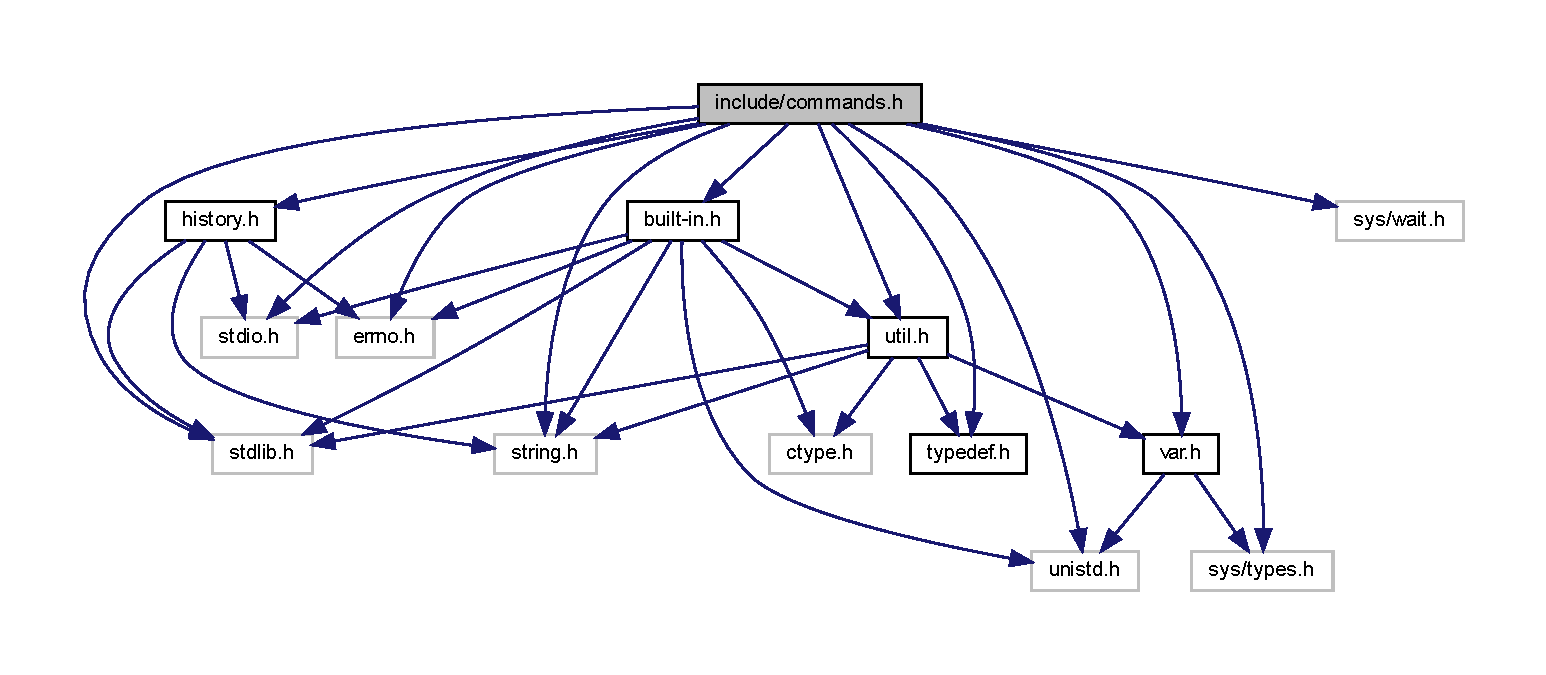
\includegraphics[width=312pt]{commands_8h__incl}
\end{center}
\end{figure}
This graph shows which files directly or indirectly include this file\+:
\nopagebreak
\begin{figure}[H]
\begin{center}
\leavevmode
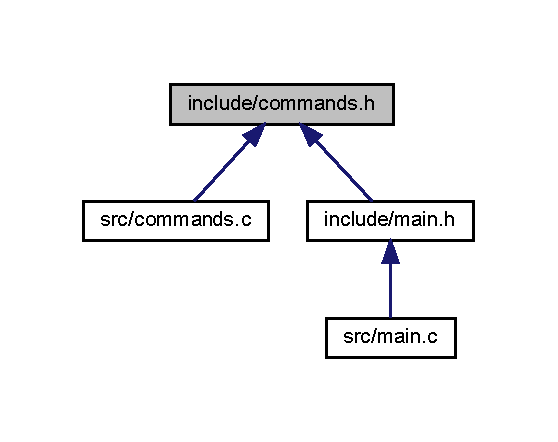
\includegraphics[width=268pt]{commands_8h__dep__incl}
\end{center}
\end{figure}
\subsection*{Functions}
\begin{DoxyCompactItemize}
\item 
void \mbox{\hyperlink{commands_8h_a21579a20737c3b2b24e18bb5e51d8140}{print\+\_\+prompt}} ()
\item 
void \mbox{\hyperlink{commands_8h_a54c8e7cbf6402612c0d796eaf3056c1f}{parse\+Command}} (char $\ast$)
\item 
void \mbox{\hyperlink{commands_8h_a7a6e0b05379c0db9c20a599404ad1bb1}{clean}} (const char $\ast$)
\item 
void \mbox{\hyperlink{commands_8h_a49f28c3d69f2302f5b4a5da84b24c581}{read\+Command}} (char $\ast$)
\end{DoxyCompactItemize}


\subsection{Function Documentation}
\mbox{\Hypertarget{commands_8h_a7a6e0b05379c0db9c20a599404ad1bb1}\label{commands_8h_a7a6e0b05379c0db9c20a599404ad1bb1}} 
\index{commands.\+h@{commands.\+h}!clean@{clean}}
\index{clean@{clean}!commands.\+h@{commands.\+h}}
\subsubsection{\texorpdfstring{clean()}{clean()}}
{\footnotesize\ttfamily void clean (\begin{DoxyParamCaption}\item[{const char $\ast$}]{buffer }\end{DoxyParamCaption})}

Clean result of fgets, remove \char`\"{}\textbackslash{}n\char`\"{} and flush stdin 
\begin{DoxyParams}{Parameters}
{\em buffer} & string to clean \\
\hline
\end{DoxyParams}

\begin{DoxyCode}
60 \{
61     \textcolor{keywordtype}{char} *p = strchr(buffer,\textcolor{charliteral}{'\(\backslash\)n'});
62     \textcolor{keywordflow}{if} (p != NULL)
63         *p = 0;
64     \textcolor{keywordflow}{else}
65     \{
66         \textcolor{keywordtype}{int} c;
67         \textcolor{keywordflow}{while} ((c = fgetc(stdin)) != \textcolor{charliteral}{'\(\backslash\)n'} && c != EOF);
68     \}
69 \}
\end{DoxyCode}
\mbox{\Hypertarget{commands_8h_a54c8e7cbf6402612c0d796eaf3056c1f}\label{commands_8h_a54c8e7cbf6402612c0d796eaf3056c1f}} 
\index{commands.\+h@{commands.\+h}!parse\+Command@{parse\+Command}}
\index{parse\+Command@{parse\+Command}!commands.\+h@{commands.\+h}}
\subsubsection{\texorpdfstring{parse\+Command()}{parseCommand()}}
{\footnotesize\ttfamily void parse\+Command (\begin{DoxyParamCaption}\item[{char $\ast$}]{command }\end{DoxyParamCaption})}

Parse the text of the command\+Line

Parse the text of the command\+Line 
\begin{DoxyParams}{Parameters}
{\em command} & command line to parse \\
\hline
\end{DoxyParams}

\begin{DoxyCode}
16 \{   
17 
18     \textcolor{comment}{// Returns first token }
19     \textcolor{keywordtype}{char} *token = strtok(command, \textcolor{stringliteral}{" "});
20    
21     \textcolor{comment}{// Keep printing tokens while one of the}
22     \textcolor{comment}{// delimiters present in str[].}
23     \textcolor{keywordflow}{while} (token != NULL)
24     \{
25         printf(\textcolor{stringliteral}{"%s\(\backslash\)n"}, token);
26         token = strtok(NULL, \textcolor{stringliteral}{" "});
27     \}
28     \textcolor{comment}{//Début d'amélioration pour le parser}
29     \textcolor{comment}{/*}
30 \textcolor{comment}{    char* word;
}
31 \textcolor{comment}{    int len = 0;
}
32 \textcolor{comment}{    printf("Caractère actuel");
}
33 \textcolor{comment}{    
}
34 \textcolor{comment}{    while(*command != '\(\backslash\)0')
}
35 \textcolor{comment}{    \{
}
36 \textcolor{comment}{        printf("Caractère actuel : %c", *command);
}
37 \textcolor{comment}{        if(*command != ' ') 
}
38 \textcolor{comment}{        \{
}
39 \textcolor{comment}{            word[len] = *command;
}
40 \textcolor{comment}{            word[len+1] = '\(\backslash\)0';
}
41 \textcolor{comment}{            len = strlen(word);
}
42 \textcolor{comment}{        \}
}
43 \textcolor{comment}{        else\{
}
44 \textcolor{comment}{            word[len+1] = '\(\backslash\)0';
}
45 \textcolor{comment}{            printf("%s\(\backslash\)n", word);
}
46 \textcolor{comment}{            len = 0;
}
47 \textcolor{comment}{            word = "";
}
48 \textcolor{comment}{        \}
}
49 \textcolor{comment}{        
}
50 \textcolor{comment}{        *command++; 
}
51 \textcolor{comment}{    \} 
}
52 \textcolor{comment}{    */}
53 \}
\end{DoxyCode}
\mbox{\Hypertarget{commands_8h_a21579a20737c3b2b24e18bb5e51d8140}\label{commands_8h_a21579a20737c3b2b24e18bb5e51d8140}} 
\index{commands.\+h@{commands.\+h}!print\+\_\+prompt@{print\+\_\+prompt}}
\index{print\+\_\+prompt@{print\+\_\+prompt}!commands.\+h@{commands.\+h}}
\subsubsection{\texorpdfstring{print\+\_\+prompt()}{print\_prompt()}}
{\footnotesize\ttfamily void print\+\_\+prompt (\begin{DoxyParamCaption}{ }\end{DoxyParamCaption})}

Prints the command lines starter 
\begin{DoxyCode}
7 \{
8     printf(\textcolor{stringliteral}{"my\_sh > "});
9 \}
\end{DoxyCode}
\mbox{\Hypertarget{commands_8h_a49f28c3d69f2302f5b4a5da84b24c581}\label{commands_8h_a49f28c3d69f2302f5b4a5da84b24c581}} 
\index{commands.\+h@{commands.\+h}!read\+Command@{read\+Command}}
\index{read\+Command@{read\+Command}!commands.\+h@{commands.\+h}}
\subsubsection{\texorpdfstring{read\+Command()}{readCommand()}}
{\footnotesize\ttfamily void read\+Command (\begin{DoxyParamCaption}\item[{char $\ast$}]{command }\end{DoxyParamCaption})}

Reads a string as a command 
\begin{DoxyParams}{Parameters}
{\em command} & string to be read as a command \\
\hline
\end{DoxyParams}

\begin{DoxyCode}
76 \{
77     \textcolor{keywordtype}{int} commandLength = strlen(command);
78 
79     \textcolor{keywordflow}{if}(commandLength > 255)
80     \{
81         printf(\textcolor{stringliteral}{"Your command exceeds 255 characters. Please enter a shorter command."});
82         exit(EXIT\_FAILURE);
83     \}
84     \textcolor{keywordflow}{else}
85     \{
86         printf(\textcolor{stringliteral}{"Your entered command: %s\(\backslash\)n"}, \mbox{\hyperlink{util_8c_ac3baffacb2ab73c47735eb93071f52c7}{stringToLower}}(command));
87     \}
88 \}
\end{DoxyCode}

\hypertarget{main_8h}{}\section{include/main.h File Reference}
\label{main_8h}\index{include/main.\+h@{include/main.\+h}}
{\ttfamily \#include $<$stdlib.\+h$>$}\newline
{\ttfamily \#include $<$stdio.\+h$>$}\newline
{\ttfamily \#include $<$string.\+h$>$}\newline
{\ttfamily \#include $<$errno.\+h$>$}\newline
{\ttfamily \#include $<$unistd.\+h$>$}\newline
{\ttfamily \#include $<$sys/types.\+h$>$}\newline
{\ttfamily \#include $<$sys/wait.\+h$>$}\newline
{\ttfamily \#include \char`\"{}commands.\+h\char`\"{}}\newline
{\ttfamily \#include \char`\"{}util.\+h\char`\"{}}\newline
Include dependency graph for main.\+h\+:
\nopagebreak
\begin{figure}[H]
\begin{center}
\leavevmode
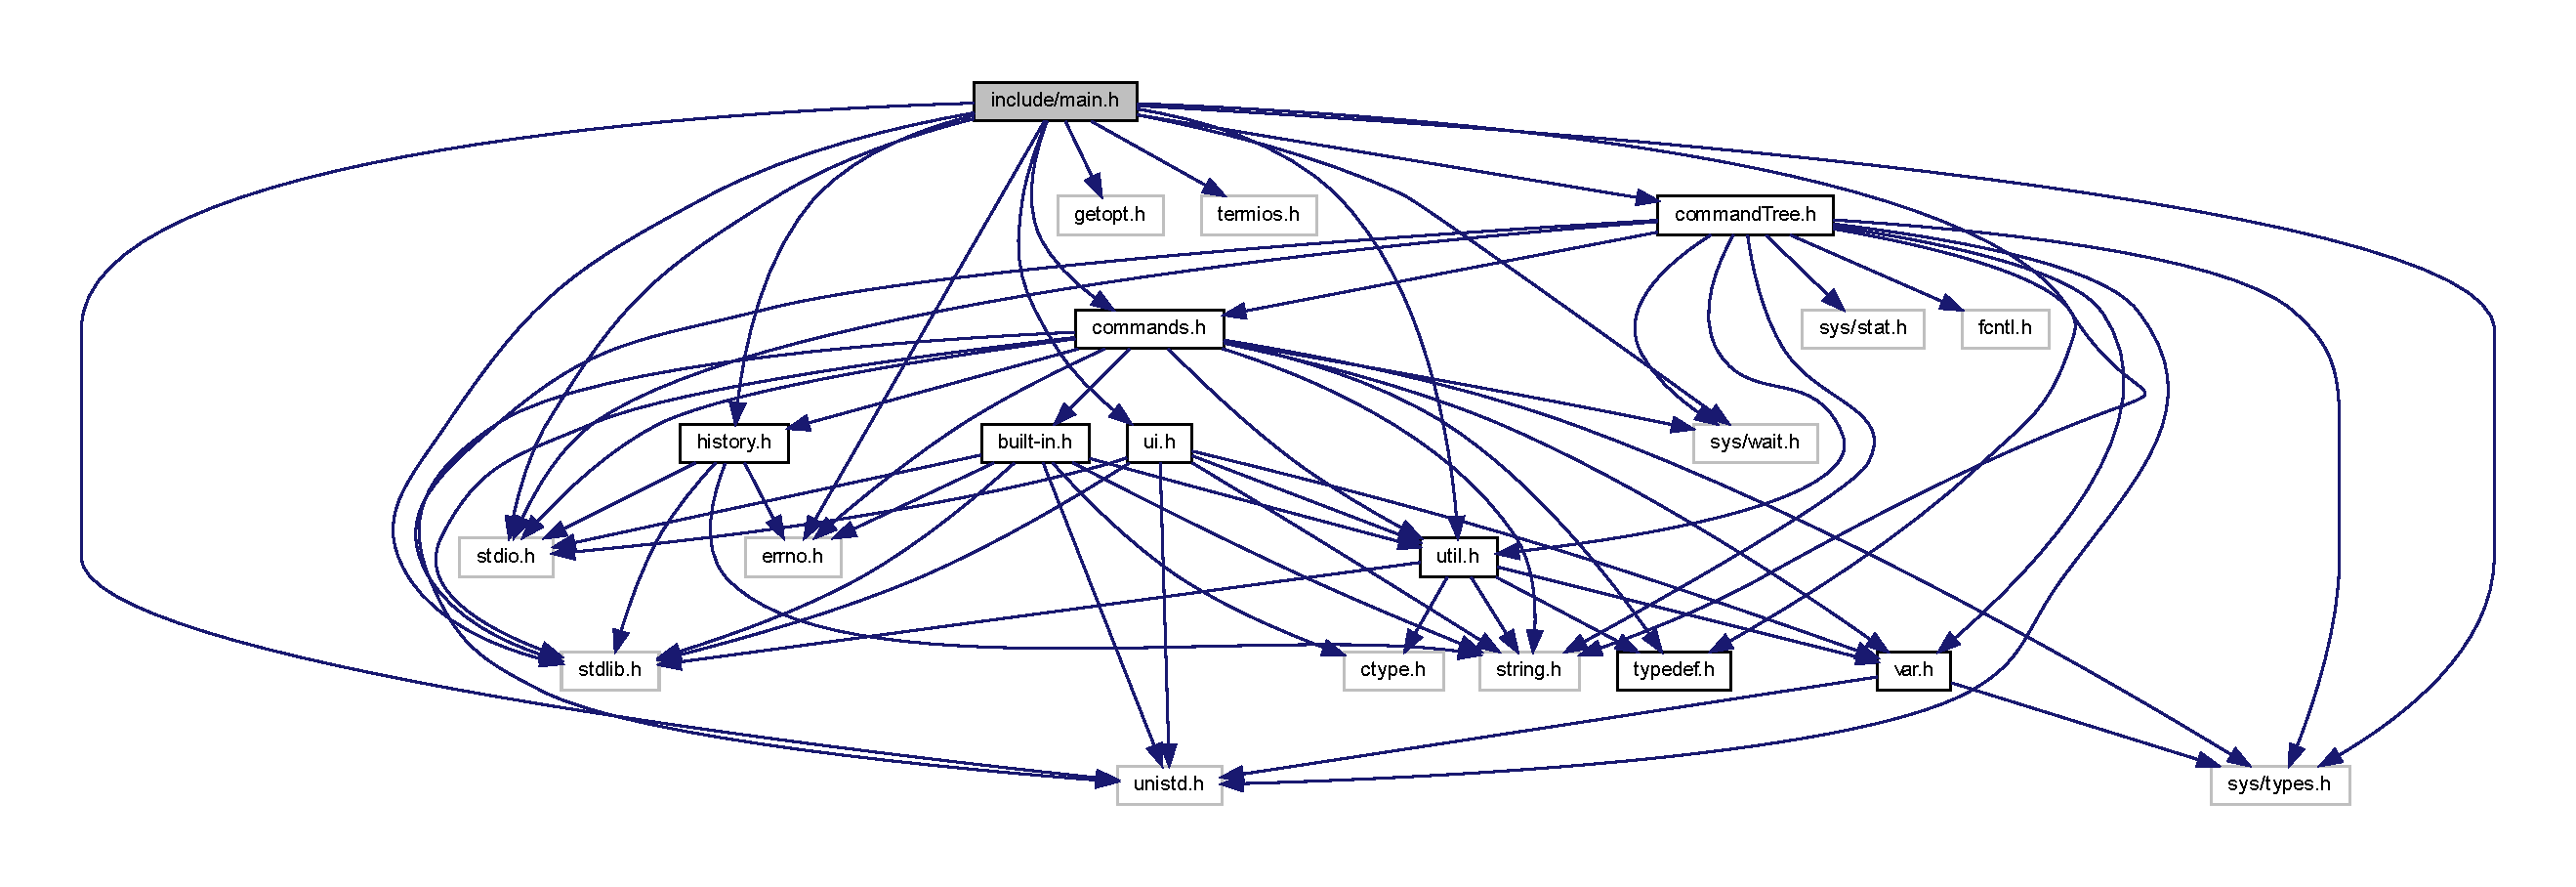
\includegraphics[width=350pt]{main_8h__incl}
\end{center}
\end{figure}
This graph shows which files directly or indirectly include this file\+:
\nopagebreak
\begin{figure}[H]
\begin{center}
\leavevmode
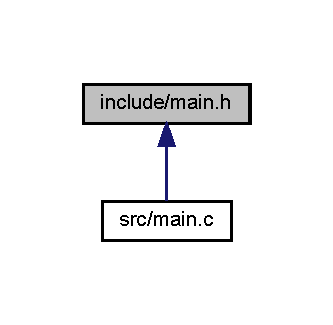
\includegraphics[width=160pt]{main_8h__dep__incl}
\end{center}
\end{figure}
\subsection*{Macros}
\begin{DoxyCompactItemize}
\item 
\#define \mbox{\hyperlink{main_8h_ad0317e5f6fe6b1e06e91cbc06dcc849d}{E\+X\+I\+T\+\_\+\+S\+T\+R\+I\+NG}}~\char`\"{}exit\char`\"{}
\end{DoxyCompactItemize}


\subsection{Macro Definition Documentation}
\mbox{\Hypertarget{main_8h_ad0317e5f6fe6b1e06e91cbc06dcc849d}\label{main_8h_ad0317e5f6fe6b1e06e91cbc06dcc849d}} 
\index{main.\+h@{main.\+h}!E\+X\+I\+T\+\_\+\+S\+T\+R\+I\+NG@{E\+X\+I\+T\+\_\+\+S\+T\+R\+I\+NG}}
\index{E\+X\+I\+T\+\_\+\+S\+T\+R\+I\+NG@{E\+X\+I\+T\+\_\+\+S\+T\+R\+I\+NG}!main.\+h@{main.\+h}}
\subsubsection{\texorpdfstring{E\+X\+I\+T\+\_\+\+S\+T\+R\+I\+NG}{EXIT\_STRING}}
{\footnotesize\ttfamily \#define E\+X\+I\+T\+\_\+\+S\+T\+R\+I\+NG~\char`\"{}exit\char`\"{}}


\hypertarget{typedef_8h}{}\section{include/typedef.h File Reference}
\label{typedef_8h}\index{include/typedef.\+h@{include/typedef.\+h}}

\hypertarget{util_8h}{}\section{include/util.h File Reference}
\label{util_8h}\index{include/util.\+h@{include/util.\+h}}
{\ttfamily \#include $<$stdlib.\+h$>$}\newline
{\ttfamily \#include $<$string.\+h$>$}\newline
{\ttfamily \#include $<$ctype.\+h$>$}\newline
{\ttfamily \#include \char`\"{}var.\+h\char`\"{}}\newline
{\ttfamily \#include \char`\"{}typedef.\+h\char`\"{}}\newline
Include dependency graph for util.\+h\+:
\nopagebreak
\begin{figure}[H]
\begin{center}
\leavevmode
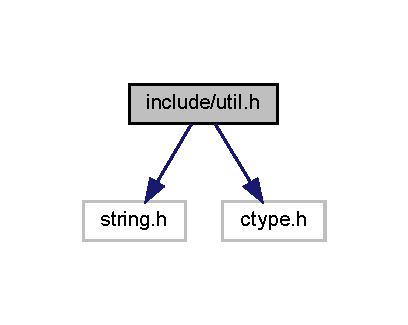
\includegraphics[width=350pt]{util_8h__incl}
\end{center}
\end{figure}
This graph shows which files directly or indirectly include this file\+:
\nopagebreak
\begin{figure}[H]
\begin{center}
\leavevmode
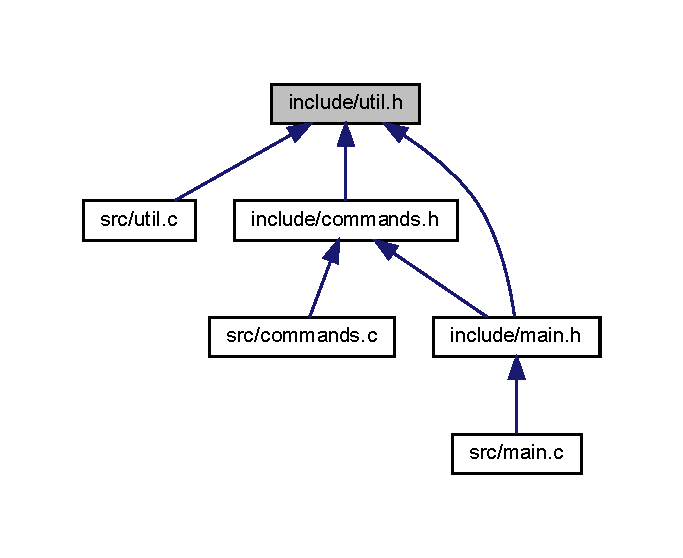
\includegraphics[width=350pt]{util_8h__dep__incl}
\end{center}
\end{figure}
\subsection*{Functions}
\begin{DoxyCompactItemize}
\item 
char $\ast$ \mbox{\hyperlink{util_8h_af309ee5385d78f13de63461ce6886a85}{string\+\_\+to\+\_\+lower}} (char $\ast$)
\item 
int \mbox{\hyperlink{util_8h_a680166b74b76fefd0e2fcf1542f950a8}{contains}} (char $\ast$str, char $\ast$seq)
\item 
int \mbox{\hyperlink{util_8h_a10bf8832498599571c7c3f108f8c41ee}{is\+Numeric}} (const char $\ast$s)
\item 
int \mbox{\hyperlink{util_8h_a2c685c7c2e8ad02b73daea6caecdf7f6}{strtonum}} (const char $\ast$str)
\item 
int \mbox{\hyperlink{util_8h_ac3d573d6edbc018dadc3e3a252444546}{strcount}} (char $\ast$str, char $\ast$search)
\item 
char $\ast$ \mbox{\hyperlink{util_8h_a7af2652d06ce1e0c36cbee5eaca5d68c}{str\+\_\+replace}} (char $\ast$search, char $\ast$replace, char $\ast$subject)
\item 
void \mbox{\hyperlink{util_8h_abee5c83f6dff2667822efe705f4d62a6}{insert\+\_\+substring}} (char $\ast$str, char $\ast$insert, int position)
\item 
char $\ast$ \mbox{\hyperlink{util_8h_a6267c19ae253842dbeeed10b3a846eb2}{substring}} (char $\ast$string, int position, int length)
\item 
char $\ast$$\ast$ \mbox{\hyperlink{util_8h_a3709c4cfc029c088669541f01f7434b2}{str\+\_\+array\+\_\+replace}} (char $\ast$$\ast$array, int size, int index\+\_\+to\+\_\+replace, char $\ast$string)
\item 
void \mbox{\hyperlink{util_8h_a6686d2dbd69aebb81a27fd296e132b07}{free\+\_\+array}} (char $\ast$$\ast$array, int array\+\_\+size)
\end{DoxyCompactItemize}


\subsection{Function Documentation}
\mbox{\Hypertarget{util_8h_a680166b74b76fefd0e2fcf1542f950a8}\label{util_8h_a680166b74b76fefd0e2fcf1542f950a8}} 
\index{util.\+h@{util.\+h}!contains@{contains}}
\index{contains@{contains}!util.\+h@{util.\+h}}
\subsubsection{\texorpdfstring{contains()}{contains()}}
{\footnotesize\ttfamily int contains (\begin{DoxyParamCaption}\item[{char $\ast$}]{str,  }\item[{char $\ast$}]{seq }\end{DoxyParamCaption})}

Indicates wether or not a string contains a certain sequence

@ param str string in which the sequence has to be searched @ param seq sequence to look for in string

\begin{DoxyReturn}{Returns}
true or false 
\end{DoxyReturn}

\begin{DoxyCode}
15 \{
16     \textcolor{keywordflow}{if} (strstr(str, seq) != NULL) \{
17         \textcolor{keywordflow}{return} \mbox{\hyperlink{var_8h_aa8cecfc5c5c054d2875c03e77b7be15d}{TRUE}};
18     \}
19     \textcolor{keywordflow}{return} \mbox{\hyperlink{var_8h_aa93f0eb578d23995850d61f7d61c55c1}{FALSE}};
20 \}
\end{DoxyCode}
\mbox{\Hypertarget{util_8h_a6686d2dbd69aebb81a27fd296e132b07}\label{util_8h_a6686d2dbd69aebb81a27fd296e132b07}} 
\index{util.\+h@{util.\+h}!free\+\_\+array@{free\+\_\+array}}
\index{free\+\_\+array@{free\+\_\+array}!util.\+h@{util.\+h}}
\subsubsection{\texorpdfstring{free\+\_\+array()}{free\_array()}}
{\footnotesize\ttfamily void free\+\_\+array (\begin{DoxyParamCaption}\item[{char $\ast$$\ast$}]{array,  }\item[{int}]{array\+\_\+size }\end{DoxyParamCaption})}

Free a char$\ast$$\ast$


\begin{DoxyParams}{Parameters}
{\em array} & the array to free \\
\hline
{\em size} & the size of the array \\
\hline
\end{DoxyParams}

\begin{DoxyCode}
230 \{
231     \textcolor{comment}{// Here we only free the array pointer}
232     \textcolor{comment}{// (we tried to free each element but we don't know why, it dumps)}
233     \textcolor{comment}{// that's why function is unsused for the moment}
234     \textcolor{keywordflow}{for}(\textcolor{keywordtype}{int} i = 0; i < array\_size; i++)
235     \{
236         free(array[i]);
237     \}
238     free(array);
239 \}
\end{DoxyCode}
\mbox{\Hypertarget{util_8h_abee5c83f6dff2667822efe705f4d62a6}\label{util_8h_abee5c83f6dff2667822efe705f4d62a6}} 
\index{util.\+h@{util.\+h}!insert\+\_\+substring@{insert\+\_\+substring}}
\index{insert\+\_\+substring@{insert\+\_\+substring}!util.\+h@{util.\+h}}
\subsubsection{\texorpdfstring{insert\+\_\+substring()}{insert\_substring()}}
{\footnotesize\ttfamily void insert\+\_\+substring (\begin{DoxyParamCaption}\item[{char $\ast$}]{str,  }\item[{char $\ast$}]{insert,  }\item[{int}]{position }\end{DoxyParamCaption})}

Inserts a string into another string at a given position


\begin{DoxyParams}{Parameters}
{\em str} & \\
\hline
{\em insert} & \\
\hline
{\em position} & \\
\hline
\end{DoxyParams}

\begin{DoxyCode}
156 \{
157    \textcolor{keywordtype}{char} *f, *e;
158    \textcolor{keywordtype}{int} length;
159  
160    length = strlen(str);
161  
162    f = \mbox{\hyperlink{util_8c_a6267c19ae253842dbeeed10b3a846eb2}{substring}}(str, 1, position - 1 ); 
163    e = \mbox{\hyperlink{util_8c_a6267c19ae253842dbeeed10b3a846eb2}{substring}}(str, position, length-position+1);
164  
165    strcpy(str, \textcolor{stringliteral}{""});
166    strcat(str, f);
167    free(f);
168    strcat(str, insert);
169    strcat(str, e);
170    free(e);
171 \}
\end{DoxyCode}
\mbox{\Hypertarget{util_8h_a10bf8832498599571c7c3f108f8c41ee}\label{util_8h_a10bf8832498599571c7c3f108f8c41ee}} 
\index{util.\+h@{util.\+h}!is\+Numeric@{is\+Numeric}}
\index{is\+Numeric@{is\+Numeric}!util.\+h@{util.\+h}}
\subsubsection{\texorpdfstring{is\+Numeric()}{isNumeric()}}
{\footnotesize\ttfamily int is\+Numeric (\begin{DoxyParamCaption}\item[{const char $\ast$}]{s }\end{DoxyParamCaption})}

Indicates wether or not a string represents a signed or unsigner numeric


\begin{DoxyParams}{Parameters}
{\em s} & string to test\\
\hline
\end{DoxyParams}
\begin{DoxyReturn}{Returns}
true if string is numeric, false otherwise 
\end{DoxyReturn}

\begin{DoxyCode}
23 \{
24     \textcolor{keywordflow}{if} (s == NULL || *s == \textcolor{charliteral}{'\(\backslash\)0'} || isspace(*s))
25       \textcolor{keywordflow}{return} 0;
26     \textcolor{keywordtype}{char} * p;
27     strtod (s, &p);
28     \textcolor{keywordflow}{return} *p == \textcolor{charliteral}{'\(\backslash\)0'};
29 \}
\end{DoxyCode}
\mbox{\Hypertarget{util_8h_a3709c4cfc029c088669541f01f7434b2}\label{util_8h_a3709c4cfc029c088669541f01f7434b2}} 
\index{util.\+h@{util.\+h}!str\+\_\+array\+\_\+replace@{str\+\_\+array\+\_\+replace}}
\index{str\+\_\+array\+\_\+replace@{str\+\_\+array\+\_\+replace}!util.\+h@{util.\+h}}
\subsubsection{\texorpdfstring{str\+\_\+array\+\_\+replace()}{str\_array\_replace()}}
{\footnotesize\ttfamily char$\ast$$\ast$ str\+\_\+array\+\_\+replace (\begin{DoxyParamCaption}\item[{char $\ast$$\ast$}]{array,  }\item[{int}]{size,  }\item[{int}]{index\+\_\+to\+\_\+replace,  }\item[{char $\ast$}]{string }\end{DoxyParamCaption})}

Replaces the value of an index into a char$\ast$$\ast$


\begin{DoxyParams}{Parameters}
{\em array} & the array to change \\
\hline
{\em size} & the size of the array \\
\hline
{\em index\+\_\+to\+\_\+replace} & the index of the array to change \\
\hline
{\em string} & the new string to put into the index\\
\hline
\end{DoxyParams}
\begin{DoxyReturn}{Returns}
a new array with the modifications 
\end{DoxyReturn}

\begin{DoxyCode}
192 \{
193     \textcolor{keywordtype}{char}** newArray  = NULL; \textcolor{comment}{// args array}
194     \textcolor{keywordtype}{int} index = 0;
195     newArray = malloc (\textcolor{keyword}{sizeof} (\textcolor{keywordtype}{char}*) * (size+1));
196     \textcolor{keywordflow}{if} (newArray == NULL) exit (-1); \textcolor{comment}{/* memory allocation failed */} 
197         
198     \textcolor{keywordtype}{char}* tmp = NULL;
199     \textcolor{comment}{// we browse the old array}
200     \textcolor{keywordflow}{while}(index < size)
201     \{
202         \textcolor{comment}{// if we aren't at the specified index, we just get the same element}
203         \textcolor{keywordflow}{if}(index != index\_to\_replace)
204         \{
205             tmp = malloc(\textcolor{keyword}{sizeof}(\textcolor{keywordtype}{char})*strlen(array[index]));
206             *tmp =\textcolor{charliteral}{'\(\backslash\)0'}; 
207             tmp = strcpy(tmp,array[index]);
208         \}
209         \textcolor{comment}{// else we get the new string}
210         \textcolor{keywordflow}{else} 
211         \{
212             tmp = malloc(\textcolor{keyword}{sizeof}(\textcolor{keywordtype}{char})*strlen(\textcolor{keywordtype}{string}));
213             *tmp = \textcolor{charliteral}{'\(\backslash\)0'};
214             tmp = strcpy(tmp,\textcolor{keywordtype}{string});
215         \}
216         
217         \textcolor{comment}{// we add the right element to the new array}
218         newArray[index] = tmp;
219         index++;    
220     \}   
221     
222     \textcolor{comment}{// we add the null, and we free the old array before to return the new one}
223     newArray[index] = 0;
224     \textcolor{comment}{//free(array);}
225 
226     \textcolor{keywordflow}{return} newArray;    
227 \}
\end{DoxyCode}
\mbox{\Hypertarget{util_8h_a7af2652d06ce1e0c36cbee5eaca5d68c}\label{util_8h_a7af2652d06ce1e0c36cbee5eaca5d68c}} 
\index{util.\+h@{util.\+h}!str\+\_\+replace@{str\+\_\+replace}}
\index{str\+\_\+replace@{str\+\_\+replace}!util.\+h@{util.\+h}}
\subsubsection{\texorpdfstring{str\+\_\+replace()}{str\_replace()}}
{\footnotesize\ttfamily char$\ast$ str\+\_\+replace (\begin{DoxyParamCaption}\item[{char $\ast$}]{search,  }\item[{char $\ast$}]{replace,  }\item[{char $\ast$}]{subject }\end{DoxyParamCaption})}

Replaces all found instances of the passed substring in the passed string.


\begin{DoxyParams}{Parameters}
{\em search} & The substring to look for \\
\hline
{\em replace} & The substring with which to replace the found substrings \\
\hline
{\em subject} & The string in which to look\\
\hline
\end{DoxyParams}
\begin{DoxyReturn}{Returns}
A new string with the search/replacement performed 
\end{DoxyReturn}
Double the size of the allocated space if it\textquotesingle{}s possible for us to surpass it

If there is a hit in characters of the substring, let\textquotesingle{}s add it to the character buffer

If the found character\textquotesingle{}s bugger\textquotesingle{}s counter has reached the searched substring\textquotesingle{}s length, then there\textquotesingle{}s a hit. Let\textquotesingle{}s copy the replace substring\textquotesingle{}s characters onto the return string.

If the character is a miss, let\textquotesingle{}s put everything back from the buffer to the return string, and set the found character buffer counter to 0.

Add the current character in the subject string to the return string.

Free memory
\begin{DoxyCode}
79                                                               \{
80     \textcolor{keywordtype}{int} i, j, k;
81     
82     \textcolor{keywordtype}{int} searchSize = strlen(search);
83     \textcolor{keywordtype}{int} replaceSize = strlen(replace);
84     \textcolor{keywordtype}{int} size = strlen(subject);
85 
86     \textcolor{keywordtype}{char}* ret;
87 
88     \textcolor{keywordflow}{if} (!searchSize) \{
89         ret = malloc(size + 1);
90         \textcolor{keywordflow}{for} (i = 0; i <= size; i++) \{
91             ret[i] = subject[i];
92         \}
93         \textcolor{keywordflow}{return} ret;
94     \}
95     
96     \textcolor{keywordtype}{int} retAllocSize = (strlen(subject) + 1) * 2; \textcolor{comment}{// Allocation size of the return string.}
97     \textcolor{comment}{// let the allocation size be twice as that of the subject initially}
98     ret = malloc(retAllocSize);
99 
100     \textcolor{keywordtype}{int} bufferSize = 0; \textcolor{comment}{// Found characters buffer counter}
101     \textcolor{keywordtype}{char}* foundBuffer = malloc(searchSize); \textcolor{comment}{// Found character bugger}
102     
103     \textcolor{keywordflow}{for} (i = 0, j = 0; i <= size; i++) \{
107         \textcolor{keywordflow}{if} (retAllocSize <= j + replaceSize) \{
108             retAllocSize *= 2;
109             ret = (\textcolor{keywordtype}{char}*) realloc(ret, retAllocSize);
110         \}
115         \textcolor{keywordflow}{else} \textcolor{keywordflow}{if} (subject[i] == search[bufferSize]) \{
116             foundBuffer[bufferSize] = subject[i];
117             bufferSize++;
118 
124             \textcolor{keywordflow}{if} (bufferSize == searchSize) \{
125                 bufferSize = 0;
126                 \textcolor{keywordflow}{for} (k = 0; k < replaceSize; k++) \{
127                     ret[j++] = replace[k];
128                 \}
129             \}
130         \}
135         \textcolor{keywordflow}{else} \{
136             \textcolor{keywordflow}{for} (k = 0; k < bufferSize; k++) \{
137                 ret[j++] = foundBuffer[k];
138             \}
139             bufferSize = 0;
143             ret[j++] = subject[i];
144         \}
145     \}
146 
150     free(foundBuffer);
151     
152     \textcolor{keywordflow}{return} ret;
153 \}
\end{DoxyCode}
\mbox{\Hypertarget{util_8h_ac3d573d6edbc018dadc3e3a252444546}\label{util_8h_ac3d573d6edbc018dadc3e3a252444546}} 
\index{util.\+h@{util.\+h}!strcount@{strcount}}
\index{strcount@{strcount}!util.\+h@{util.\+h}}
\subsubsection{\texorpdfstring{strcount()}{strcount()}}
{\footnotesize\ttfamily int strcount (\begin{DoxyParamCaption}\item[{char $\ast$}]{str,  }\item[{char $\ast$}]{search }\end{DoxyParamCaption})}

Count occurences of a certain character in a string


\begin{DoxyParams}{Parameters}
{\em str} & string to look into \\
\hline
{\em search} & char seq to find and count\\
\hline
\end{DoxyParams}
\begin{DoxyReturn}{Returns}
count 
\end{DoxyReturn}

\begin{DoxyCode}
48 \{
49     \textcolor{keywordtype}{int} i, j, found, count;
50     \textcolor{keywordtype}{int} stringLen, searchLen;
51 
52     stringLen = strlen(str);      \textcolor{comment}{// length of string}
53     searchLen = strlen(search); \textcolor{comment}{// length of word to be searched}
54 
55     count = 0;
56 
57     \textcolor{keywordflow}{for}(i=0; i <= stringLen-searchLen; i++)
58     \{
59         \textcolor{comment}{/* Match word with string */}
60         found = 1;
61         \textcolor{keywordflow}{for}(j=0; j<searchLen; j++)
62         \{
63             \textcolor{keywordflow}{if}(str[i + j] != search[j])
64             \{
65                 found = 0;
66                 \textcolor{keywordflow}{break};
67             \}
68         \}
69 
70         \textcolor{keywordflow}{if}(found == 1)
71         \{
72             count++;
73         \}
74     \}
75 
76     \textcolor{keywordflow}{return} count;
77 \}
\end{DoxyCode}
\mbox{\Hypertarget{util_8h_af309ee5385d78f13de63461ce6886a85}\label{util_8h_af309ee5385d78f13de63461ce6886a85}} 
\index{util.\+h@{util.\+h}!string\+\_\+to\+\_\+lower@{string\+\_\+to\+\_\+lower}}
\index{string\+\_\+to\+\_\+lower@{string\+\_\+to\+\_\+lower}!util.\+h@{util.\+h}}
\subsubsection{\texorpdfstring{string\+\_\+to\+\_\+lower()}{string\_to\_lower()}}
{\footnotesize\ttfamily char$\ast$ string\+\_\+to\+\_\+lower (\begin{DoxyParamCaption}\item[{char $\ast$}]{ }\end{DoxyParamCaption})}

Returns a string in lower case


\begin{DoxyParams}{Parameters}
{\em string} & string to be returned in lower case\\
\hline
\end{DoxyParams}
\begin{DoxyReturn}{Returns}
string in lower-\/case 
\end{DoxyReturn}

\begin{DoxyCode}
5 \{
6     \textcolor{keywordflow}{for}(\textcolor{keywordtype}{int} i = 0; i < strlen(\textcolor{keywordtype}{string}); i++)
7     \{
8         \textcolor{keywordtype}{string}[i] = tolower(\textcolor{keywordtype}{string}[i]);
9     \}
10 
11     \textcolor{keywordflow}{return} string;
12 \}
\end{DoxyCode}
\mbox{\Hypertarget{util_8h_a2c685c7c2e8ad02b73daea6caecdf7f6}\label{util_8h_a2c685c7c2e8ad02b73daea6caecdf7f6}} 
\index{util.\+h@{util.\+h}!strtonum@{strtonum}}
\index{strtonum@{strtonum}!util.\+h@{util.\+h}}
\subsubsection{\texorpdfstring{strtonum()}{strtonum()}}
{\footnotesize\ttfamily int strtonum (\begin{DoxyParamCaption}\item[{const char $\ast$}]{str }\end{DoxyParamCaption})}

Converts a string to an integer


\begin{DoxyParams}{Parameters}
{\em str} & string to convert\\
\hline
\end{DoxyParams}
\begin{DoxyReturn}{Returns}
resulting integer 
\end{DoxyReturn}

\begin{DoxyCode}
32 \{
33     \textcolor{keywordtype}{int}  i, len;
34 
35     \textcolor{keywordtype}{int} result = 0;
36 
37     len = strlen(str);
38 
39     \textcolor{keywordflow}{for}(i = 0; i < len; i++)
40     \{
41         result = result * 10 + ( str[i] - \textcolor{charliteral}{'0'} );
42     \}
43 
44     \textcolor{keywordflow}{return} result;
45 \}
\end{DoxyCode}
\mbox{\Hypertarget{util_8h_a6267c19ae253842dbeeed10b3a846eb2}\label{util_8h_a6267c19ae253842dbeeed10b3a846eb2}} 
\index{util.\+h@{util.\+h}!substring@{substring}}
\index{substring@{substring}!util.\+h@{util.\+h}}
\subsubsection{\texorpdfstring{substring()}{substring()}}
{\footnotesize\ttfamily char$\ast$ substring (\begin{DoxyParamCaption}\item[{char $\ast$}]{string,  }\item[{int}]{position,  }\item[{int}]{length }\end{DoxyParamCaption})}

Gets substring


\begin{DoxyParams}{Parameters}
{\em string} & string from which we want a substring \\
\hline
{\em position} & start index \\
\hline
{\em length} & end index from position\\
\hline
\end{DoxyParams}
\begin{DoxyReturn}{Returns}
substring 
\end{DoxyReturn}

\begin{DoxyCode}
174 \{
175    \textcolor{keywordtype}{char} *pointer;
176    \textcolor{keywordtype}{int} c;
177  
178    pointer = malloc(length+1);
179  
180    \textcolor{keywordflow}{if}( pointer == NULL )
181        exit(EXIT\_FAILURE);
182  
183    \textcolor{keywordflow}{for}( c = 0 ; c < length ; c++ ) 
184       *(pointer+c) = *((\textcolor{keywordtype}{string}+position-1)+c);       
185  
186    *(pointer+c) = \textcolor{charliteral}{'\(\backslash\)0'};
187  
188    \textcolor{keywordflow}{return} pointer;
189 \}
\end{DoxyCode}

\hypertarget{commands_8c}{}\section{src/commands.c File Reference}
\label{commands_8c}\index{src/commands.\+c@{src/commands.\+c}}
{\ttfamily \#include \char`\"{}commands.\+h\char`\"{}}\newline
Include dependency graph for commands.\+c\+:
\nopagebreak
\begin{figure}[H]
\begin{center}
\leavevmode
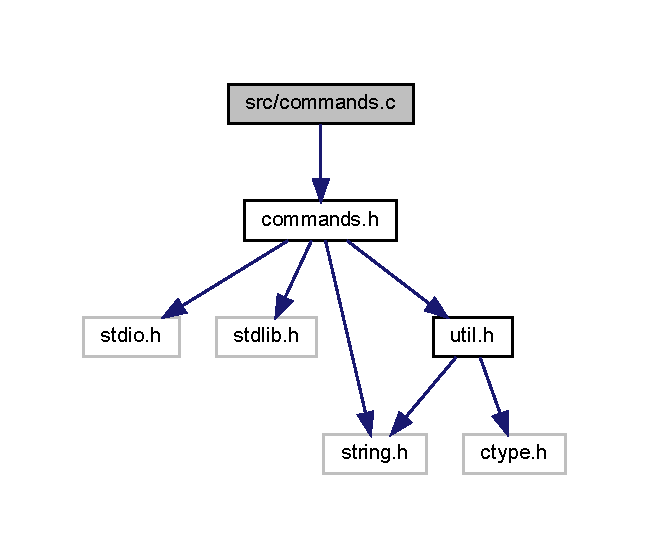
\includegraphics[width=350pt]{commands_8c__incl}
\end{center}
\end{figure}
\subsection*{Functions}
\begin{DoxyCompactItemize}
\item 
char $\ast$$\ast$ \mbox{\hyperlink{commands_8c_ac08a987d5042f86c1de985c6c24fe300}{parse\+\_\+to\+\_\+argv}} (char $\ast$command, int $\ast$argc)
\item 
char $\ast$$\ast$ \mbox{\hyperlink{commands_8c_aeb88ec8a1adef5cbcd9d8de252aa5475}{interpret\+\_\+heard\+\_\+file}} (char $\ast$$\ast$argv, int args\+\_\+count)
\item 
int \mbox{\hyperlink{commands_8c_a5cdbb99fa3ac8fa9ab9394f4e563995f}{execute\+\_\+command}} (char $\ast$$\ast$argv, int argc)
\item 
int \mbox{\hyperlink{commands_8c_a1586f3c18d7c2dc8c65687c90678b6fe}{execute\+\_\+builtin}} (char $\ast$$\ast$argv, int argc)
\item 
int \mbox{\hyperlink{commands_8c_aea90c4618f1ea3d250aa2189888b0829}{isbuiltin}} (char $\ast$command\+Line)
\item 
int \mbox{\hyperlink{commands_8c_a75057c1eff6e3decd05f01997f381b5e}{includes\+\_\+multplie\+\_\+commands}} (char $\ast$$\ast$argv, int argc)
\item 
char $\ast$$\ast$ \mbox{\hyperlink{commands_8c_ad0a7668bf0100523d1bc449de6ab123c}{get\+\_\+next\+\_\+command\+\_\+args}} (char $\ast$$\ast$argv, int argc, int $\ast$nxt\+\_\+argc, int $\ast$nxt\+Cmd\+Line\+Index)
\item 
char $\ast$$\ast$ \mbox{\hyperlink{commands_8c_a36a2466ea1a146371efe4974eb5d4b22}{get\+\_\+last\+\_\+command\+\_\+args}} (char $\ast$$\ast$argv, int argc, int $\ast$last\+\_\+argc, int start\+Index)
\end{DoxyCompactItemize}
\subsection*{Variables}
\begin{DoxyCompactItemize}
\item 
const char $\ast$ \mbox{\hyperlink{commands_8c_ab6e3c2ad539285b3027db5fa1903ee00}{built\+\_\+in\+\_\+commands}} \mbox{[}$\,$\mbox{]} = \{\char`\"{}cd\char`\"{}, \char`\"{}\mbox{\hyperlink{built-in_8h_a7f540865bf44effc4cd5f843a0d29388}{pwd}}\char`\"{}, \char`\"{}\mbox{\hyperlink{built-in_8h_ae985125913017d37bb75b1ab7b977950}{echo}}\char`\"{}, \char`\"{}exit\char`\"{}\}
\item 
int \mbox{\hyperlink{commands_8c_a1a7dcdfeabbc3dc651e199403984d99e}{n\+\_\+built\+\_\+in}} = sizeof(\mbox{\hyperlink{commands_8c_ab6e3c2ad539285b3027db5fa1903ee00}{built\+\_\+in\+\_\+commands}}) / sizeof(const char$\ast$)
\end{DoxyCompactItemize}


\subsection{Function Documentation}
\mbox{\Hypertarget{commands_8c_a1586f3c18d7c2dc8c65687c90678b6fe}\label{commands_8c_a1586f3c18d7c2dc8c65687c90678b6fe}} 
\index{commands.\+c@{commands.\+c}!execute\+\_\+builtin@{execute\+\_\+builtin}}
\index{execute\+\_\+builtin@{execute\+\_\+builtin}!commands.\+c@{commands.\+c}}
\subsubsection{\texorpdfstring{execute\+\_\+builtin()}{execute\_builtin()}}
{\footnotesize\ttfamily int execute\+\_\+builtin (\begin{DoxyParamCaption}\item[{char $\ast$$\ast$}]{args,  }\item[{int}]{argc }\end{DoxyParamCaption})}

Executes a buitl-\/in command using argv and argc


\begin{DoxyParams}{Parameters}
{\em argv} & array of arguments \\
\hline
{\em argc} & arguments count\\
\hline
\end{DoxyParams}
\begin{DoxyReturn}{Returns}
0 on success, -\/1 on failure 
\end{DoxyReturn}

\begin{DoxyCode}
257 \{
258     \textcolor{keywordtype}{int} returnCode;
259 
260     \textcolor{keywordflow}{if}(!\mbox{\hyperlink{commands_8c_aea90c4618f1ea3d250aa2189888b0829}{isbuiltin}}(argv[0]))
261     \{
262         returnCode = -1;
263     \}
264     \textcolor{keywordflow}{else} \textcolor{keywordflow}{if}(strcmp(argv[0],\textcolor{stringliteral}{"cd"}) == 0)
265     \{
266         returnCode = \mbox{\hyperlink{built-in_8c_a6e03260ed7d8b2ac33c1116c55c2cec7}{cd}}(argv,argc);
267     \}
268     \textcolor{keywordflow}{else} \textcolor{keywordflow}{if}(strcmp(argv[0],\textcolor{stringliteral}{"pwd"}) == 0)
269     \{
270         returnCode = \mbox{\hyperlink{built-in_8c_a7f540865bf44effc4cd5f843a0d29388}{pwd}}(argv,argc);
271     \}
272     \textcolor{keywordflow}{else} \textcolor{keywordflow}{if}(strcmp(argv[0],\textcolor{stringliteral}{"echo"}) == 0)
273     \{
274         returnCode = \mbox{\hyperlink{built-in_8c_ae985125913017d37bb75b1ab7b977950}{echo}}(argv,argc);
275     \}
276     \textcolor{keywordflow}{else} \textcolor{keywordflow}{if}(strcmp(argv[0],\textcolor{stringliteral}{"exit"}) == 0)
277     \{
278         \mbox{\hyperlink{built-in_8c_a203155f52ab90e655b8040e61130dbcc}{builtin\_exit}}(argv,argc);
279     \}
280 
281     printf(\textcolor{stringliteral}{"\(\backslash\)n"});
282 
283     \textcolor{keywordflow}{return} returnCode;
284 \}
\end{DoxyCode}
\mbox{\Hypertarget{commands_8c_a5cdbb99fa3ac8fa9ab9394f4e563995f}\label{commands_8c_a5cdbb99fa3ac8fa9ab9394f4e563995f}} 
\index{commands.\+c@{commands.\+c}!execute\+\_\+command@{execute\+\_\+command}}
\index{execute\+\_\+command@{execute\+\_\+command}!commands.\+c@{commands.\+c}}
\subsubsection{\texorpdfstring{execute\+\_\+command()}{execute\_command()}}
{\footnotesize\ttfamily int execute\+\_\+command (\begin{DoxyParamCaption}\item[{char $\ast$$\ast$}]{argv,  }\item[{int}]{argc }\end{DoxyParamCaption})}

Executes a command using argv and argc


\begin{DoxyParams}{Parameters}
{\em argv} & array of arguments \\
\hline
{\em argc} & arguments count\\
\hline
\end{DoxyParams}
\begin{DoxyReturn}{Returns}
the exit code of process 
\end{DoxyReturn}

\begin{DoxyCode}
165 \{
166     \textcolor{comment}{// case built-in command}
167     \textcolor{keywordflow}{if}(\mbox{\hyperlink{commands_8c_aea90c4618f1ea3d250aa2189888b0829}{isbuiltin}}(argv[0]))
168     \{
169         \textcolor{keywordflow}{return} \mbox{\hyperlink{commands_8c_a1586f3c18d7c2dc8c65687c90678b6fe}{execute\_builtin}}(argv, argc);
170     \}
171     \textcolor{comment}{// other commands}
172     \textcolor{keywordflow}{else}
173     \{
174         \textcolor{comment}{// fork}
175         \textcolor{keywordtype}{int} pid;
176         \textcolor{keywordtype}{int} status;
177         \textcolor{keywordflow}{if} ((pid = fork()) < 0)
178         \{
179             perror(\textcolor{stringliteral}{"fork"});
180             exit(EXIT\_FAILURE);
181         \}
182 
183         \textcolor{comment}{// child}
184         \textcolor{keywordflow}{if}(pid == 0)
185         \{
186             \textcolor{comment}{// buidling the path}
187             \textcolor{keywordtype}{char}* bin = \textcolor{stringliteral}{"/bin/"};
188             \textcolor{keywordtype}{char}* path = malloc(strlen(bin) * \textcolor{keyword}{sizeof}(\textcolor{keywordtype}{char})) + ((strlen(argv[0]) + 1) * \textcolor{keyword}{sizeof}(\textcolor{keywordtype}{char}));
189             *path = \textcolor{charliteral}{'\(\backslash\)0'};
190             path = strcat(path,bin);
191             path = strcat(path,argv[0]);
192             
193             \textcolor{comment}{// execution}
194             \textcolor{keywordflow}{if} (execvp(path, argv) == -1) \{
195                 \textcolor{keywordflow}{if}(errno == ENOENT)
196                 \{
197                     fprintf(stderr,\textcolor{stringliteral}{"%s: Command not found\(\backslash\)n"},argv[0]);
198                 \}
199                 \textcolor{keywordflow}{else}
200                 \{
201                     perror(argv[0]);
202                 \}
203                 exit(-1);
204             \}
205         \}
206         \textcolor{comment}{// parent}
207         \textcolor{keywordflow}{else}
208         \{
209             wait(&status);
210             \textcolor{keywordflow}{if}(WIFEXITED(status) && WEXITSTATUS(status) == 0) 
211             \{
212                 \textcolor{keywordflow}{return} status;
213             \}
214             \textcolor{keywordflow}{return} -1;
215         \}
216         
217     \}
218     \textcolor{keywordflow}{return} -1;
219     
220     \textcolor{comment}{/*if(argv[0] == NULL)
}
221 \textcolor{comment}{    \{
}
222 \textcolor{comment}{        return;
}
223 \textcolor{comment}{    \}
}
224 \textcolor{comment}{    
}
225 \textcolor{comment}{    else if(isbuiltin(argv[0]))
}
226 \textcolor{comment}{    \{
}
227 \textcolor{comment}{        if(execute\_builtin(argv,argc) == 0) exit(EXIT\_SUCCESS);
}
228 \textcolor{comment}{        else exit(EXIT\_FAILURE);
}
229 \textcolor{comment}{    \}
}
230 \textcolor{comment}{}
231 \textcolor{comment}{    char* bin = "/bin/";
}
232 \textcolor{comment}{    char* path = malloc(strlen(bin) * sizeof(char)) + ((strlen(argv[0]) + 1) * sizeof(char));
}
233 \textcolor{comment}{    strcat(path,bin);
}
234 \textcolor{comment}{    strcat(path,argv[0]);
}
235 \textcolor{comment}{}
236 \textcolor{comment}{    if (execvp(path, argv) == -1) \{
}
237 \textcolor{comment}{        if(errno == ENOENT)
}
238 \textcolor{comment}{        \{
}
239 \textcolor{comment}{            fprintf(stderr,"%s: Command not found\(\backslash\)n",argv[0]);
}
240 \textcolor{comment}{        \}
}
241 \textcolor{comment}{        else
}
242 \textcolor{comment}{        \{
}
243 \textcolor{comment}{            perror(argv[0]);
}
244 \textcolor{comment}{        \}
}
245 \textcolor{comment}{        free(path);
}
246 \textcolor{comment}{        exit(EXIT\_FAILURE);
}
247 \textcolor{comment}{    \}
}
248 \textcolor{comment}{}
249 \textcolor{comment}{    printf("\(\backslash\)n\(\backslash\)n");
}
250 \textcolor{comment}{}
251 \textcolor{comment}{    free(path);
}
252 \textcolor{comment}{    */}
253 
254 \}
\end{DoxyCode}
\mbox{\Hypertarget{commands_8c_a36a2466ea1a146371efe4974eb5d4b22}\label{commands_8c_a36a2466ea1a146371efe4974eb5d4b22}} 
\index{commands.\+c@{commands.\+c}!get\+\_\+last\+\_\+command\+\_\+args@{get\+\_\+last\+\_\+command\+\_\+args}}
\index{get\+\_\+last\+\_\+command\+\_\+args@{get\+\_\+last\+\_\+command\+\_\+args}!commands.\+c@{commands.\+c}}
\subsubsection{\texorpdfstring{get\+\_\+last\+\_\+command\+\_\+args()}{get\_last\_command\_args()}}
{\footnotesize\ttfamily char$\ast$$\ast$ get\+\_\+last\+\_\+command\+\_\+args (\begin{DoxyParamCaption}\item[{char $\ast$$\ast$}]{argv,  }\item[{int}]{argc,  }\item[{int $\ast$}]{last\+\_\+argc,  }\item[{int}]{start\+Index }\end{DoxyParamCaption})}

Gets the last sequence of commands that has to be ran (i.\+e. if there were any \textquotesingle{};\textquotesingle{}, gets the last sequence after the last \textquotesingle{};\textquotesingle{})


\begin{DoxyParams}{Parameters}
{\em argv} & array of arguments \\
\hline
{\em argc} & arguments count (input arguments array) \\
\hline
{\em last\+\_\+argc} & arguments count (output arguments array) \\
\hline
{\em start\+Index} & \\
\hline
\end{DoxyParams}
\begin{DoxyReturn}{Returns}
sub-\/array of arguments to be used 
\end{DoxyReturn}

\begin{DoxyCode}
343 \{
344     \textcolor{keywordtype}{char}** last\_argv = NULL;
345 
346     \textcolor{keywordtype}{int} n\_args = 0;
347 
348     \textcolor{comment}{// We copy all the arguments at the end (after all the ; operators)}
349     \textcolor{keywordflow}{for}(\textcolor{keywordtype}{int} i = startIndex; i < argc; i++)
350     \{
351         \textcolor{comment}{// reallocating memory}
352         last\_argv = realloc(last\_argv, \textcolor{keyword}{sizeof} (\textcolor{keywordtype}{char}*) * ++n\_args);
353         \textcolor{keywordflow}{if} (last\_argv == NULL) exit (-1); \textcolor{comment}{/* memory allocation failed */}
354 
355         last\_argv[n\_args - 1] = argv[i];
356     \}
357 
358     \textcolor{comment}{/* realloc one extra element for the last NULL 
}
359 \textcolor{comment}{     (necessary for exec fucntion)*/}
360     last\_argv = realloc (last\_argv, \textcolor{keyword}{sizeof} (\textcolor{keywordtype}{char}*) * (n\_args+1));
361     last\_argv[n\_args] = 0;
362 
363     *last\_argc = n\_args;
364 
365     \textcolor{keywordflow}{return} last\_argv;
366 \}
\end{DoxyCode}
\mbox{\Hypertarget{commands_8c_ad0a7668bf0100523d1bc449de6ab123c}\label{commands_8c_ad0a7668bf0100523d1bc449de6ab123c}} 
\index{commands.\+c@{commands.\+c}!get\+\_\+next\+\_\+command\+\_\+args@{get\+\_\+next\+\_\+command\+\_\+args}}
\index{get\+\_\+next\+\_\+command\+\_\+args@{get\+\_\+next\+\_\+command\+\_\+args}!commands.\+c@{commands.\+c}}
\subsubsection{\texorpdfstring{get\+\_\+next\+\_\+command\+\_\+args()}{get\_next\_command\_args()}}
{\footnotesize\ttfamily char$\ast$$\ast$ get\+\_\+next\+\_\+command\+\_\+args (\begin{DoxyParamCaption}\item[{char $\ast$$\ast$}]{argv,  }\item[{int}]{argc,  }\item[{int $\ast$}]{nxt\+\_\+argc,  }\item[{int $\ast$}]{nxt\+Cmd\+Line\+Index }\end{DoxyParamCaption})}

Gets the next sequence of commands after \textquotesingle{};\textquotesingle{}


\begin{DoxyParams}{Parameters}
{\em argv} & array of arguments \\
\hline
{\em argc} & arguments count (input arguments array) \\
\hline
{\em nxt\+\_\+argc} & arguments count (output arguments array) \\
\hline
{\em nxt\+Cmd\+Line\+Index} & index of the next command line (after \& operator)\\
\hline
\end{DoxyParams}
\begin{DoxyReturn}{Returns}
array of arguments to be used 
\end{DoxyReturn}

\begin{DoxyCode}
312 \{
313     \textcolor{keywordtype}{char}** nxt\_argv = NULL;
314 
315     \textcolor{keywordtype}{int} n\_args = 0;
316     \textcolor{keywordtype}{int} i = *nxtCmdLineIndex;
317 
318     \textcolor{comment}{// We copy all the arguments to get only the ones concerned by the next ; operator}
319     \textcolor{keywordflow}{while}(strcmp(argv[i],\textcolor{stringliteral}{";"}) != 0)
320     \{
321         \textcolor{comment}{// reallocating memory}
322         nxt\_argv = realloc(nxt\_argv, \textcolor{keyword}{sizeof} (\textcolor{keywordtype}{char}*) * ++n\_args);
323         \textcolor{keywordflow}{if} (nxt\_argv == NULL) exit (-1); \textcolor{comment}{/* memory allocation failed */}
324 
325         nxt\_argv[n\_args - 1] = argv[i];
326         i++;
327     \}
328     \textcolor{comment}{// Sets ";" to "" in argv}
329     argv[i] = \textcolor{stringliteral}{""};
330     *nxtCmdLineIndex = i + 1;
331 
332     \textcolor{comment}{/* realloc one extra element for the last NULL 
}
333 \textcolor{comment}{     (necessary for exec fucntion)*/}
334     nxt\_argv = realloc (nxt\_argv, \textcolor{keyword}{sizeof} (\textcolor{keywordtype}{char}*) * (n\_args+1));
335     nxt\_argv[n\_args] = 0;
336 
337     *nxt\_argc = n\_args;
338 
339     \textcolor{keywordflow}{return} nxt\_argv;
340 \}
\end{DoxyCode}
\mbox{\Hypertarget{commands_8c_a75057c1eff6e3decd05f01997f381b5e}\label{commands_8c_a75057c1eff6e3decd05f01997f381b5e}} 
\index{commands.\+c@{commands.\+c}!includes\+\_\+multplie\+\_\+commands@{includes\+\_\+multplie\+\_\+commands}}
\index{includes\+\_\+multplie\+\_\+commands@{includes\+\_\+multplie\+\_\+commands}!commands.\+c@{commands.\+c}}
\subsubsection{\texorpdfstring{includes\+\_\+multplie\+\_\+commands()}{includes\_multplie\_commands()}}
{\footnotesize\ttfamily int includes\+\_\+multplie\+\_\+commands (\begin{DoxyParamCaption}\item[{char $\ast$$\ast$}]{argv,  }\item[{int}]{argc }\end{DoxyParamCaption})}

Indicates wether or not a command line (parsed into argv) includes multiple command(s) (i.\+e. separated by ;).


\begin{DoxyParams}{Parameters}
{\em argv} & array of arguments \\
\hline
{\em argc} & arguments count\\
\hline
\end{DoxyParams}
\begin{DoxyReturn}{Returns}
true if argv contains at least one ; and false otherwise 
\end{DoxyReturn}

\begin{DoxyCode}
299 \{
300     \textcolor{keywordflow}{for}(\textcolor{keywordtype}{int} i = 0; i < argc; i++)
301     \{
302         \textcolor{keywordflow}{if}(strcmp(argv[i],\textcolor{stringliteral}{";"}) == 0)
303         \{
304             \textcolor{keywordflow}{return} \mbox{\hyperlink{var_8h_aa8cecfc5c5c054d2875c03e77b7be15d}{TRUE}};
305         \}
306     \}
307 
308     \textcolor{keywordflow}{return} \mbox{\hyperlink{var_8h_aa93f0eb578d23995850d61f7d61c55c1}{FALSE}};
309 \}
\end{DoxyCode}
\mbox{\Hypertarget{commands_8c_aeb88ec8a1adef5cbcd9d8de252aa5475}\label{commands_8c_aeb88ec8a1adef5cbcd9d8de252aa5475}} 
\index{commands.\+c@{commands.\+c}!interpret\+\_\+heard\+\_\+file@{interpret\+\_\+heard\+\_\+file}}
\index{interpret\+\_\+heard\+\_\+file@{interpret\+\_\+heard\+\_\+file}!commands.\+c@{commands.\+c}}
\subsubsection{\texorpdfstring{interpret\+\_\+heard\+\_\+file()}{interpret\_heard\_file()}}
{\footnotesize\ttfamily char$\ast$$\ast$ interpret\+\_\+heard\+\_\+file (\begin{DoxyParamCaption}\item[{char $\ast$$\ast$}]{argv,  }\item[{int}]{args\+\_\+count }\end{DoxyParamCaption})}

Interprets symbols \char`\"{}$<$$<$\char`\"{} of the command line, creates a tmp file it pattern is \+: \char`\"{}/tmp/tmp\+Shell\+X\+X\+X\+X\+X\+X.\+tmp\char`\"{} it contains what the user typed until he wrote the delimiter the delimiter is replace by the tmp file path


\begin{DoxyParams}{Parameters}
{\em argv} & array of arguments \\
\hline
{\em args\+\_\+count} & arguments count\\
\hline
\end{DoxyParams}
\begin{DoxyReturn}{Returns}
the new array of arguments 
\end{DoxyReturn}

\begin{DoxyCode}
85 \{
86     \textcolor{keywordtype}{int} index = 0;
87     
88     \textcolor{comment}{// brownsing the entire command}
89     \textcolor{keywordflow}{while}(index < args\_count)
90     \{
91         \textcolor{comment}{// case a "<<" is find}
92         \textcolor{keywordflow}{if}(strcmp(\textcolor{stringliteral}{"<<"}, argv[index]) == 0)
93         \{
94             
95             \textcolor{keywordtype}{char} line\_input[\mbox{\hyperlink{var_8h_a0592dba56693fad79136250c11e5a7fe}{MAX\_SIZE}}];
96             \textcolor{keywordtype}{char}* stdin\_text = malloc(\textcolor{keyword}{sizeof}(\textcolor{keywordtype}{char}));
97             *stdin\_text = \textcolor{charliteral}{'\(\backslash\)0'};
98 
99             \textcolor{keywordflow}{if}(argv[index+1] == NULL)
100             \{
101                 fprintf(stderr,\textcolor{stringliteral}{"bash: syntax error near unexpected token '<<'\(\backslash\)n"});
102                 \textcolor{keywordflow}{return} argv;
103             \}
104             \textcolor{keywordtype}{char}* delimiter = malloc(strlen(argv[index+1])*\textcolor{keyword}{sizeof}((\textcolor{keywordtype}{char}) + 1));
105             
106             delimiter = strcpy(delimiter, argv[index+1]);
107             delimiter = strcat(delimiter,\textcolor{stringliteral}{"\(\backslash\)n"});  \textcolor{comment}{// adding a \(\backslash\)n to the delimiter  (in order to be able to
       compare it with fget)}
108             
109             \textcolor{comment}{// letting the user write some lines until he writes the delimiter after << }
110             \textcolor{keywordflow}{do}
111             \{
112                 printf(\textcolor{stringliteral}{" > "});
113                 fgets(line\_input, \textcolor{keyword}{sizeof}(line\_input), stdin);
114                 
115                 \textcolor{keywordflow}{if}(strcmp(delimiter, line\_input) != 0)
116                 \{
117                     \textcolor{keywordtype}{int} spaceNeeded = ((strlen(stdin\_text)) * \textcolor{keyword}{sizeof}(\textcolor{keywordtype}{char})) + ((strlen(line\_input) + 3) * \textcolor{keyword}{
      sizeof}(\textcolor{keywordtype}{char}));
118                     stdin\_text = realloc(stdin\_text,spaceNeeded);
119                     stdin\_text = strcat(stdin\_text, line\_input);
120                 \}   
121             \} \textcolor{keywordflow}{while}(strcmp(delimiter, line\_input) != 0);
122             
123             \mbox{\hyperlink{history_8c_ad048e165fa6cd1fbc4bbc3fc8baac839}{write\_to\_history}}(stdin\_text);
124             free(delimiter);
125             
126             \textcolor{comment}{// creating a temporary files (which will be readed during the execution of the tree    }
127             \textcolor{keywordtype}{int} descTemp;
128             \textcolor{keyword}{static} \textcolor{keywordtype}{char} \textcolor{keyword}{template}[] = \textcolor{stringliteral}{"/tmp/tmpShellXXXXXX.txt"};
129             \textcolor{keywordtype}{char} fileName[23];
130             
131             strcpy(fileName, \textcolor{keyword}{template});
132             
133             descTemp = mkstemps(fileName,4);
134             \textcolor{keywordflow}{if}(descTemp == -1) \{
135                 perror(\textcolor{stringliteral}{"error !"});
136                 dprintf(\mbox{\hyperlink{var_8h_a3a540e3eef339eec06aff31c4ba1eb25}{STDERR}}, \textcolor{stringliteral}{"Error in mkstemp.\(\backslash\)n"});
137                 exit(EXIT\_FAILURE);
138             \}
139             
140             \textcolor{comment}{// writing what the user wrote before into the tmp file}
141             FILE *fp = fdopen(descTemp, \textcolor{stringliteral}{"w"});
142             \textcolor{keywordflow}{if} (fp == NULL)
143             \{
144                 perror(\textcolor{stringliteral}{"Error when opening temp file"});
145                 exit(EXIT\_FAILURE);
146             \}
147             
148             fputs(stdin\_text, fp);
149             
150             \textcolor{comment}{// replacing  the delimiter by the tmp file path}
151             \textcolor{keywordtype}{char}* tmp = malloc(\textcolor{keyword}{sizeof}(\textcolor{keywordtype}{char}) * strlen(fileName));
152             strcpy(tmp, fileName);
153             argv = \mbox{\hyperlink{util_8c_a3709c4cfc029c088669541f01f7434b2}{str\_array\_replace}}(argv, args\_count,(index+1), tmp);
154             
155             fclose(fp);
156             close(descTemp);
157             free(stdin\_text);
158         \}
159         index++;
160     \}
161     \textcolor{keywordflow}{return} argv;
162 \}
\end{DoxyCode}
\mbox{\Hypertarget{commands_8c_aea90c4618f1ea3d250aa2189888b0829}\label{commands_8c_aea90c4618f1ea3d250aa2189888b0829}} 
\index{commands.\+c@{commands.\+c}!isbuiltin@{isbuiltin}}
\index{isbuiltin@{isbuiltin}!commands.\+c@{commands.\+c}}
\subsubsection{\texorpdfstring{isbuiltin()}{isbuiltin()}}
{\footnotesize\ttfamily int isbuiltin (\begin{DoxyParamCaption}\item[{char $\ast$}]{command\+Line }\end{DoxyParamCaption})}

Indicates wether or not the command is a built-\/in command


\begin{DoxyParams}{Parameters}
{\em command\+Line} & \\
\hline
\end{DoxyParams}
\begin{DoxyReturn}{Returns}
true or false 
\end{DoxyReturn}

\begin{DoxyCode}
287 \{
288     \textcolor{keywordflow}{for}(\textcolor{keywordtype}{int} i = 0; i < \mbox{\hyperlink{commands_8c_a1a7dcdfeabbc3dc651e199403984d99e}{n\_built\_in}}; i++)
289     \{
290         \textcolor{keywordflow}{if}(strcmp(commandLine,\mbox{\hyperlink{commands_8c_ab6e3c2ad539285b3027db5fa1903ee00}{built\_in\_commands}}[i]) == 0)
291         \{
292             \textcolor{keywordflow}{return} \mbox{\hyperlink{var_8h_aa8cecfc5c5c054d2875c03e77b7be15d}{TRUE}};
293         \}
294     \}
295     \textcolor{keywordflow}{return} \mbox{\hyperlink{var_8h_aa93f0eb578d23995850d61f7d61c55c1}{FALSE}};
296 \}
\end{DoxyCode}
\mbox{\Hypertarget{commands_8c_ac08a987d5042f86c1de985c6c24fe300}\label{commands_8c_ac08a987d5042f86c1de985c6c24fe300}} 
\index{commands.\+c@{commands.\+c}!parse\+\_\+to\+\_\+argv@{parse\+\_\+to\+\_\+argv}}
\index{parse\+\_\+to\+\_\+argv@{parse\+\_\+to\+\_\+argv}!commands.\+c@{commands.\+c}}
\subsubsection{\texorpdfstring{parse\+\_\+to\+\_\+argv()}{parse\_to\_argv()}}
{\footnotesize\ttfamily char$\ast$$\ast$ parse\+\_\+to\+\_\+argv (\begin{DoxyParamCaption}\item[{char $\ast$}]{,  }\item[{int $\ast$}]{ }\end{DoxyParamCaption})}

Parses the text of the command\+Line


\begin{DoxyParams}{Parameters}
{\em command} & command line to parse \\
\hline
{\em argc} & argument count \\
\hline
\end{DoxyParams}

\begin{DoxyCode}
7 \{
8     \textcolor{keywordtype}{char}** argv  = NULL; \textcolor{comment}{// args array}
9     \textcolor{keywordtype}{char} *  p    = strtok (command, \textcolor{stringliteral}{" "}); \textcolor{comment}{// token}
10     \textcolor{keywordtype}{int} n\_spaces = 0; \textcolor{comment}{// args counter}
11 
12     \textcolor{keywordtype}{int} awaitingClosingQuote = \mbox{\hyperlink{var_8h_aa93f0eb578d23995850d61f7d61c55c1}{FALSE}}; \textcolor{comment}{// indicates wether or not quote is opened and not closed}
13     \textcolor{keywordtype}{char}* tmp = \textcolor{stringliteral}{""}; \textcolor{comment}{// hold between quotes string until closing quote reached}
14 
15 
16     \textcolor{comment}{/* split string and append tokens to 'argv' */}
17 
18     \textcolor{keywordflow}{while} (p) \{
19         \textcolor{comment}{// reallocating memory as the arg count augments}
20         \textcolor{comment}{// (only reallocating once if arg between quotes, i.e. spaces ignored)}
21         \textcolor{keywordflow}{if}(awaitingClosingQuote != \mbox{\hyperlink{var_8h_aa8cecfc5c5c054d2875c03e77b7be15d}{TRUE}}) argv = realloc (argv, \textcolor{keyword}{sizeof} (\textcolor{keywordtype}{char}*) * ++n\_spaces);
22 
23         \textcolor{keywordflow}{if} (argv == NULL) exit (-1); \textcolor{comment}{/* memory allocation failed */}
24 
25         \textcolor{comment}{// if still waiting for closing quote}
26         \textcolor{keywordflow}{if}(awaitingClosingQuote == \mbox{\hyperlink{var_8h_aa8cecfc5c5c054d2875c03e77b7be15d}{TRUE}})
27         \{
28             \textcolor{keywordtype}{int} spaceNeeded = (strlen(tmp) * \textcolor{keyword}{sizeof}(char)) + ((strlen(p) + 1) * \textcolor{keyword}{sizeof}(\textcolor{keywordtype}{char})) + 1;
29             tmp = realloc(tmp,spaceNeeded);
30             strcat(tmp,\textcolor{stringliteral}{" "});
31             strcat(tmp,p);
32         \}
33 
34         \textcolor{comment}{// if current argument starts with quotes}
35         \textcolor{keywordflow}{if}((p[0] == \textcolor{charliteral}{'"'}) && (awaitingClosingQuote != \mbox{\hyperlink{var_8h_aa8cecfc5c5c054d2875c03e77b7be15d}{TRUE}}))
36         \{
37             \textcolor{comment}{// only one word between quotes = normal token}
38             \textcolor{keywordflow}{if}(p[strlen(p) - 1] == \textcolor{charliteral}{'"'})
39             \{
40                 p = \mbox{\hyperlink{util_8c_a7af2652d06ce1e0c36cbee5eaca5d68c}{str\_replace}}(\textcolor{stringliteral}{"\(\backslash\)""},\textcolor{stringliteral}{""},p);
41                 argv[n\_spaces-1] = p;
42                 p = strtok (NULL, \textcolor{stringliteral}{" "});
43                 \textcolor{keywordflow}{continue};
44             \}
45 
46             \textcolor{comment}{// initiates tmp string to hold string between quotes}
47             awaitingClosingQuote = \mbox{\hyperlink{var_8h_aa8cecfc5c5c054d2875c03e77b7be15d}{TRUE}};
48             tmp = strdup(p);
49             p = strtok(NULL, \textcolor{stringliteral}{" "});
50             \textcolor{keywordflow}{continue};
51         \}
52         \textcolor{comment}{// if closing quote is reached}
53         \textcolor{keywordflow}{else} \textcolor{keywordflow}{if}((p[strlen(p) - 1] == \textcolor{charliteral}{'"'}) && (awaitingClosingQuote == \mbox{\hyperlink{var_8h_aa8cecfc5c5c054d2875c03e77b7be15d}{TRUE}}))
54         \{
55             awaitingClosingQuote = \mbox{\hyperlink{var_8h_aa93f0eb578d23995850d61f7d61c55c1}{FALSE}};
56             tmp = \mbox{\hyperlink{util_8c_a7af2652d06ce1e0c36cbee5eaca5d68c}{str\_replace}}(\textcolor{stringliteral}{"\(\backslash\)""},\textcolor{stringliteral}{""},tmp);
57             argv[n\_spaces-1] = tmp;
58             p = strtok(NULL, \textcolor{stringliteral}{" "});
59             tmp = \textcolor{stringliteral}{""};
60             \textcolor{keywordflow}{continue};
61         \}
62         \textcolor{comment}{// end of command string is reached while still waiting for closing quote}
63         \textcolor{keywordflow}{else} \textcolor{keywordflow}{if}((awaitingClosingQuote == \mbox{\hyperlink{var_8h_aa8cecfc5c5c054d2875c03e77b7be15d}{TRUE}}) && (p[strlen(p)] == \textcolor{charliteral}{'\(\backslash\)0'}))
64         \{
65             argv[n\_spaces-1] = tmp;
66             p = strtok(NULL, \textcolor{stringliteral}{" "});
67             \textcolor{keywordflow}{continue};
68         \}   
69         
70         argv[n\_spaces-1] = p;
71         p = strtok (NULL, \textcolor{stringliteral}{" "});
72     \}
73 
74     \textcolor{comment}{/* realloc one extra element for the last NULL 
}
75 \textcolor{comment}{     (necessary for exec fucntion)*/}
76     argv = realloc (argv, \textcolor{keyword}{sizeof} (\textcolor{keywordtype}{char}*) * (n\_spaces+1));
77     argv[n\_spaces] = 0;
78 
79     *argc = n\_spaces;
80     
81     \textcolor{keywordflow}{return} argv;
82 \}
\end{DoxyCode}


\subsection{Variable Documentation}
\mbox{\Hypertarget{commands_8c_ab6e3c2ad539285b3027db5fa1903ee00}\label{commands_8c_ab6e3c2ad539285b3027db5fa1903ee00}} 
\index{commands.\+c@{commands.\+c}!built\+\_\+in\+\_\+commands@{built\+\_\+in\+\_\+commands}}
\index{built\+\_\+in\+\_\+commands@{built\+\_\+in\+\_\+commands}!commands.\+c@{commands.\+c}}
\subsubsection{\texorpdfstring{built\+\_\+in\+\_\+commands}{built\_in\_commands}}
{\footnotesize\ttfamily const char$\ast$ built\+\_\+in\+\_\+commands\mbox{[}$\,$\mbox{]} = \{\char`\"{}cd\char`\"{}, \char`\"{}\mbox{\hyperlink{built-in_8h_a7f540865bf44effc4cd5f843a0d29388}{pwd}}\char`\"{}, \char`\"{}\mbox{\hyperlink{built-in_8h_ae985125913017d37bb75b1ab7b977950}{echo}}\char`\"{}, \char`\"{}exit\char`\"{}\}}

\mbox{\Hypertarget{commands_8c_a1a7dcdfeabbc3dc651e199403984d99e}\label{commands_8c_a1a7dcdfeabbc3dc651e199403984d99e}} 
\index{commands.\+c@{commands.\+c}!n\+\_\+built\+\_\+in@{n\+\_\+built\+\_\+in}}
\index{n\+\_\+built\+\_\+in@{n\+\_\+built\+\_\+in}!commands.\+c@{commands.\+c}}
\subsubsection{\texorpdfstring{n\+\_\+built\+\_\+in}{n\_built\_in}}
{\footnotesize\ttfamily int n\+\_\+built\+\_\+in = sizeof(\mbox{\hyperlink{commands_8c_ab6e3c2ad539285b3027db5fa1903ee00}{built\+\_\+in\+\_\+commands}}) / sizeof(const char$\ast$)}


\hypertarget{main_8c}{}\section{src/main.c File Reference}
\label{main_8c}\index{src/main.\+c@{src/main.\+c}}
{\ttfamily \#include \char`\"{}main.\+h\char`\"{}}\newline
Include dependency graph for main.\+c\+:
\nopagebreak
\begin{figure}[H]
\begin{center}
\leavevmode
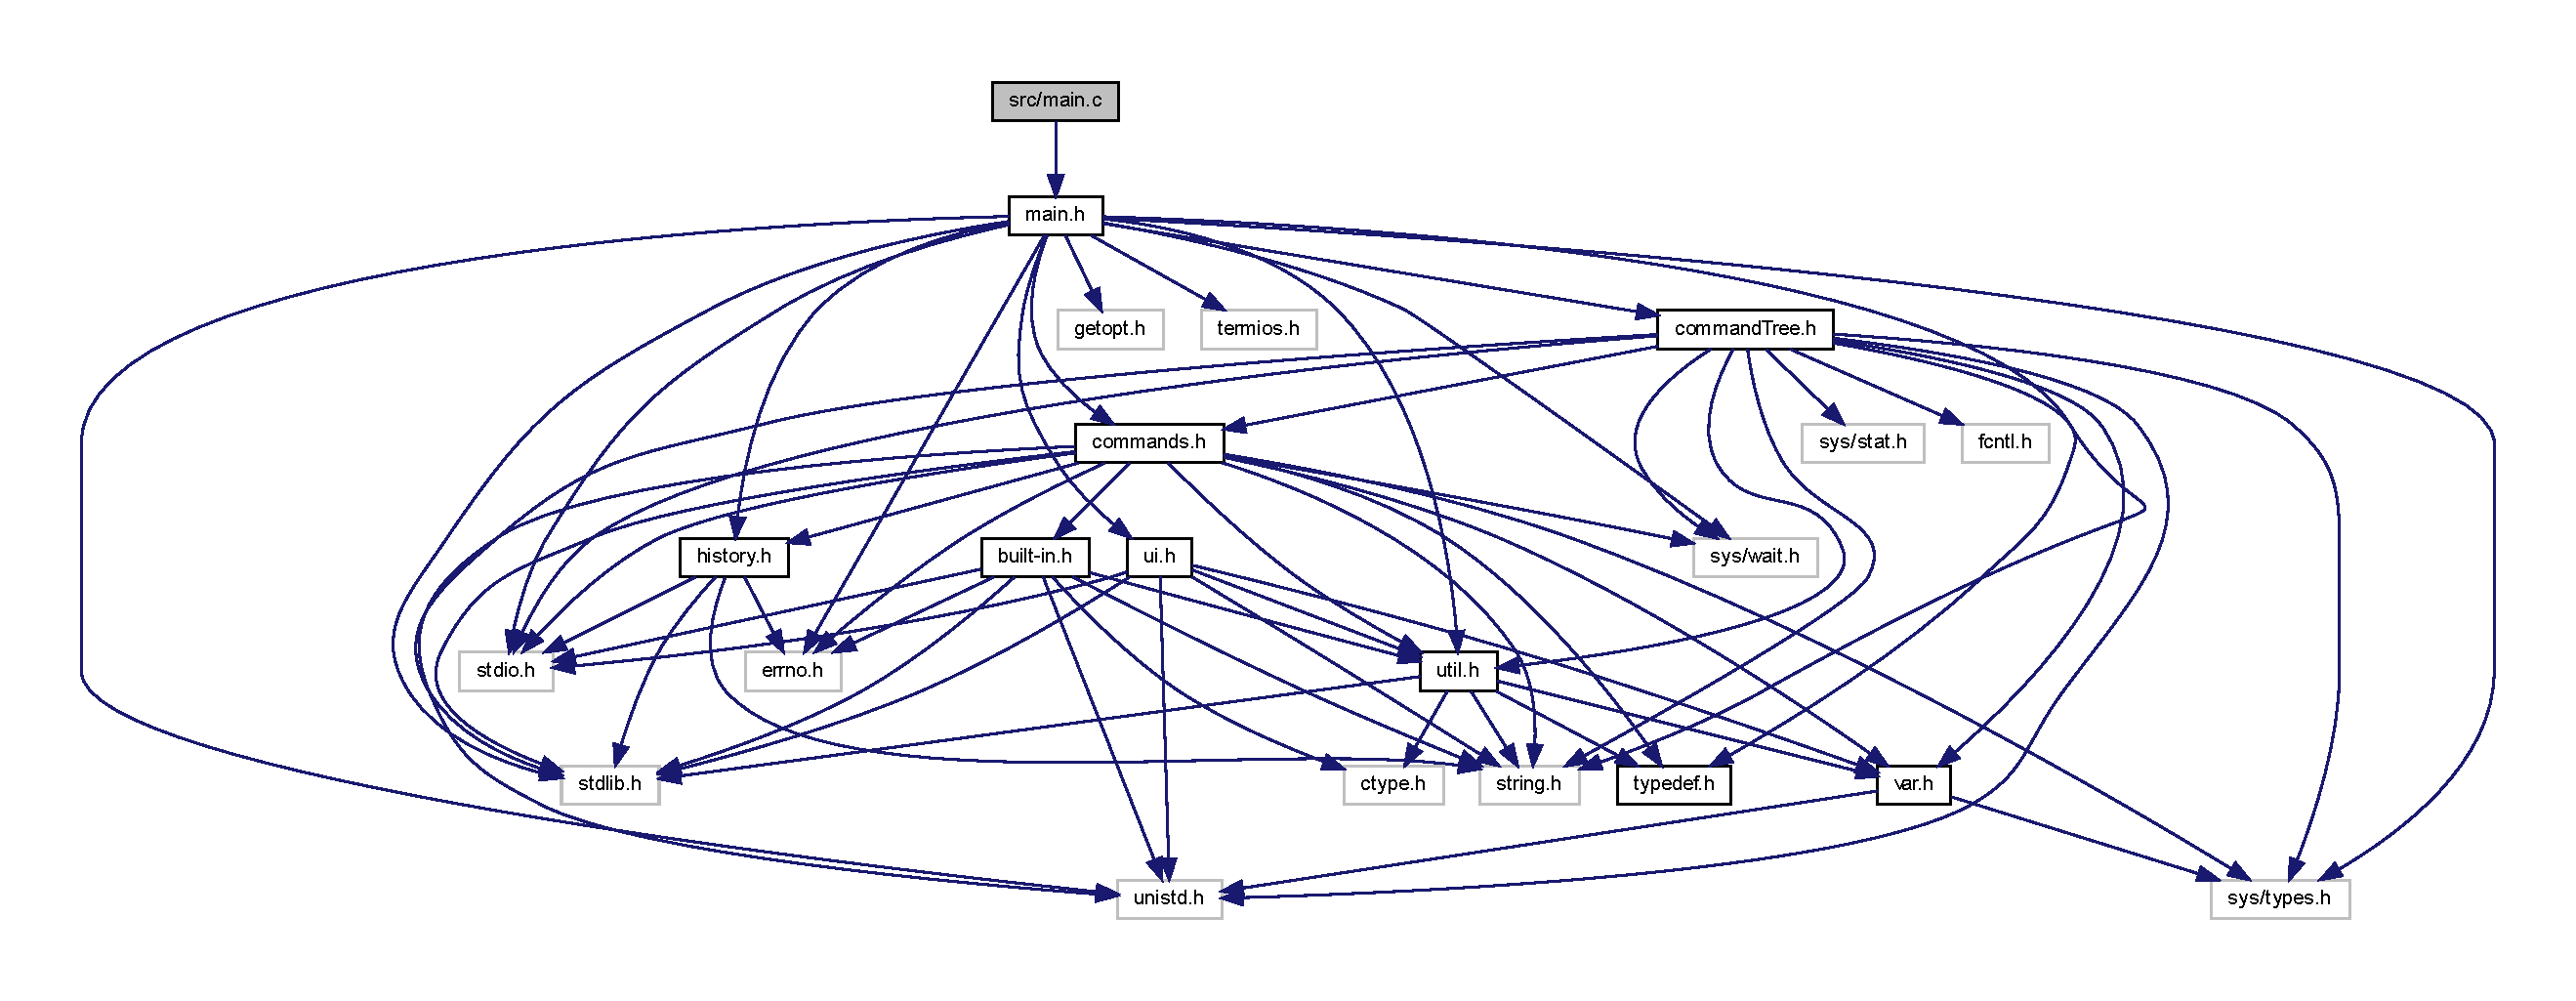
\includegraphics[width=350pt]{main_8c__incl}
\end{center}
\end{figure}
\subsection*{Functions}
\begin{DoxyCompactItemize}
\item 
void \mbox{\hyperlink{main_8c_a2ceab08439bad173313751f2f3b6475c}{print\+\_\+usage}} (char $\ast$bin\+\_\+name)
\item 
void \mbox{\hyperlink{main_8c_a21a43e2b75ce805de38950c1f4ccdc91}{free\+\_\+if\+\_\+needed}} (void $\ast$to\+\_\+free)
\item 
char $\ast$ \mbox{\hyperlink{main_8c_a3003fdfd0b79fc3effcf9cd81d2f5890}{dup\+\_\+optarg\+\_\+str}} ()
\item 
void \mbox{\hyperlink{main_8c_ab5e54de1ad77145e82c60a2fdbb80c86}{process\+\_\+command\+\_\+line}} (char $\ast$command\+Line)
\item 
void \mbox{\hyperlink{main_8c_ae22e556dbb94b941317c1e93265c2bb4}{execute\+\_\+command\+\_\+line}} (char $\ast$$\ast$argv, int argc, int is\+Background)
\item 
void \mbox{\hyperlink{main_8c_a9b9d7c6b417dcda5bd5d53d11fcaa2d8}{exit\+\_\+prog}} (char $\ast$bin\+\_\+command\+\_\+param, int code)
\item 
int \mbox{\hyperlink{main_8c_a3c04138a5bfe5d72780bb7e82a18e627}{main}} (int argc, char $\ast$$\ast$argv)
\end{DoxyCompactItemize}


\subsection{Function Documentation}
\mbox{\Hypertarget{main_8c_a3003fdfd0b79fc3effcf9cd81d2f5890}\label{main_8c_a3003fdfd0b79fc3effcf9cd81d2f5890}} 
\index{main.\+c@{main.\+c}!dup\+\_\+optarg\+\_\+str@{dup\+\_\+optarg\+\_\+str}}
\index{dup\+\_\+optarg\+\_\+str@{dup\+\_\+optarg\+\_\+str}!main.\+c@{main.\+c}}
\subsubsection{\texorpdfstring{dup\+\_\+optarg\+\_\+str()}{dup\_optarg\_str()}}
{\footnotesize\ttfamily char$\ast$ dup\+\_\+optarg\+\_\+str (\begin{DoxyParamCaption}{ }\end{DoxyParamCaption})}

\begin{DoxySeeAlso}{See also}
man 3 strndup 

man 3 perror 
\end{DoxySeeAlso}
\begin{DoxyReturn}{Returns}

\end{DoxyReturn}

\begin{DoxyCode}
14 \{
15   \textcolor{keywordtype}{char}* str = NULL;
16 
17   \textcolor{keywordflow}{if} (optarg != NULL)
18   \{
19     str = strndup(optarg, \mbox{\hyperlink{var_8h_a0592dba56693fad79136250c11e5a7fe}{MAX\_SIZE}});
20     
21     \textcolor{comment}{// Checking if ERRNO is set}
22     \textcolor{keywordflow}{if} (str == NULL) 
23       perror(strerror(errno));
24   \}
25 
26   \textcolor{keywordflow}{return} str;
27 \}
\end{DoxyCode}
\mbox{\Hypertarget{main_8c_ae22e556dbb94b941317c1e93265c2bb4}\label{main_8c_ae22e556dbb94b941317c1e93265c2bb4}} 
\index{main.\+c@{main.\+c}!execute\+\_\+command\+\_\+line@{execute\+\_\+command\+\_\+line}}
\index{execute\+\_\+command\+\_\+line@{execute\+\_\+command\+\_\+line}!main.\+c@{main.\+c}}
\subsubsection{\texorpdfstring{execute\+\_\+command\+\_\+line()}{execute\_command\_line()}}
{\footnotesize\ttfamily void execute\+\_\+command\+\_\+line (\begin{DoxyParamCaption}\item[{char $\ast$$\ast$}]{argv,  }\item[{int}]{argc,  }\item[{int}]{is\+Background }\end{DoxyParamCaption})}

Execute a command line 
\begin{DoxyParams}{Parameters}
{\em argv} & array of arguments \\
\hline
{\em argc} & arguments count \\
\hline
{\em is\+Background} & wether or not the process has to be ran in background \\
\hline
\end{DoxyParams}

\begin{DoxyCode}
111 \{
112     \mbox{\hyperlink{structcommandNode}{commandNode}}* tree\_arguments = \mbox{\hyperlink{commandTree_8c_a26b3f0fbe7d40e8de4f2900641a30ef4}{parse\_to\_tree}}(argv, argc);
113     
114     \mbox{\hyperlink{commandTree_8c_a56ed6b9afd9134e7d57be5fd60562d5d}{execute\_tree}}(tree\_arguments,isBackground);
115 
116     \textcolor{comment}{// int status;}
117     \textcolor{comment}{// pid\_t pid;}
118     \textcolor{comment}{// while((pid = waitpid(-1, NULL, WNOHANG)) > 0) \{}
119     \textcolor{comment}{//     printf("[process %d exited with code %d]\(\backslash\)n",}
120     \textcolor{comment}{//     pid, WEXITSTATUS(status));}
121     \textcolor{comment}{//     /* here you can remove the pid from your jobs list */}
122     \textcolor{comment}{//     int i = 0;}
123     \textcolor{comment}{//     while(BG\_PIDS\_ARRAY[i] != 0)}
124     \textcolor{comment}{//     \{}
125     \textcolor{comment}{//         if(BG\_PIDS\_ARRAY[i] == pid)}
126     \textcolor{comment}{//         \{}
127     \textcolor{comment}{//             BG\_PIDS\_ARRAY[i] = 0;}
128     \textcolor{comment}{//             break;}
129     \textcolor{comment}{//         \}}
130     \textcolor{comment}{//         i++;}
131     \textcolor{comment}{//     \}}
132     \textcolor{comment}{// \}}
133 
134     \mbox{\hyperlink{commandTree_8c_ab553fb78bed7105079a8c557226b9676}{free\_tree}}(tree\_arguments);
135 
136     free(argv);
137 \}
\end{DoxyCode}
\mbox{\Hypertarget{main_8c_a9b9d7c6b417dcda5bd5d53d11fcaa2d8}\label{main_8c_a9b9d7c6b417dcda5bd5d53d11fcaa2d8}} 
\index{main.\+c@{main.\+c}!exit\+\_\+prog@{exit\+\_\+prog}}
\index{exit\+\_\+prog@{exit\+\_\+prog}!main.\+c@{main.\+c}}
\subsubsection{\texorpdfstring{exit\+\_\+prog()}{exit\_prog()}}
{\footnotesize\ttfamily void exit\+\_\+prog (\begin{DoxyParamCaption}\item[{char $\ast$}]{bin\+\_\+command\+\_\+param,  }\item[{int}]{code }\end{DoxyParamCaption})}

Exits the program 
\begin{DoxyCode}
140 \{
141    \textcolor{comment}{// Freeing allocated data}
142     \mbox{\hyperlink{main_8c_a21a43e2b75ce805de38950c1f4ccdc91}{free\_if\_needed}}(bin\_command\_param);
143     \textcolor{comment}{// Exiting with a failure ERROR CODE (== 1)}
144     exit(code);
145 \}
\end{DoxyCode}
\mbox{\Hypertarget{main_8c_a21a43e2b75ce805de38950c1f4ccdc91}\label{main_8c_a21a43e2b75ce805de38950c1f4ccdc91}} 
\index{main.\+c@{main.\+c}!free\+\_\+if\+\_\+needed@{free\+\_\+if\+\_\+needed}}
\index{free\+\_\+if\+\_\+needed@{free\+\_\+if\+\_\+needed}!main.\+c@{main.\+c}}
\subsubsection{\texorpdfstring{free\+\_\+if\+\_\+needed()}{free\_if\_needed()}}
{\footnotesize\ttfamily void free\+\_\+if\+\_\+needed (\begin{DoxyParamCaption}\item[{void $\ast$}]{to\+\_\+free }\end{DoxyParamCaption})}

Procedure checks if variable must be free (check\+: ptr != N\+U\+LL)


\begin{DoxyParams}{Parameters}
{\em void$\ast$} & to\+\_\+free pointer to an allocated mem \\
\hline
\end{DoxyParams}
\begin{DoxySeeAlso}{See also}
man 3 free 
\end{DoxySeeAlso}
\begin{DoxyReturn}{Returns}
void 
\end{DoxyReturn}

\begin{DoxyCode}
9 \{
10   \textcolor{keywordflow}{if} (to\_free != NULL) free(to\_free);  
11 \}
\end{DoxyCode}
\mbox{\Hypertarget{main_8c_a3c04138a5bfe5d72780bb7e82a18e627}\label{main_8c_a3c04138a5bfe5d72780bb7e82a18e627}} 
\index{main.\+c@{main.\+c}!main@{main}}
\index{main@{main}!main.\+c@{main.\+c}}
\subsubsection{\texorpdfstring{main()}{main()}}
{\footnotesize\ttfamily int main (\begin{DoxyParamCaption}\item[{int}]{argc,  }\item[{char $\ast$$\ast$}]{argv }\end{DoxyParamCaption})}

Progam 
\begin{DoxyParams}{Parameters}
{\em argc} & arguments count \\
\hline
{\em argv} & array of arguments \\
\hline
\end{DoxyParams}
Binary variables

Checking binary requirements
\begin{DoxyCode}
153 \{
154 
158     \textcolor{keywordtype}{char}* bin\_command\_param = NULL;
159 
160     \textcolor{comment}{// Parsing options}
161     \textcolor{keywordtype}{int} opt = -1;
162     \textcolor{keywordtype}{int} opt\_idx = -1;
163 
164     \textcolor{keywordflow}{while} ((opt = getopt\_long(argc, argv, \mbox{\hyperlink{main_8h_a97fc43177532913a1d7408f2bca3b7ef}{binary\_optstr}}, 
      \mbox{\hyperlink{main_8h_a853665eee6ed9fc2ad8d5f44956e5e3f}{binary\_opts}}, &opt\_idx)) != -1)
165     \{
166         \textcolor{keywordflow}{switch} (opt)
167         \{
168             \textcolor{keywordflow}{case} \textcolor{charliteral}{'c'}:
169                 \textcolor{comment}{//input param}
170                 \textcolor{keywordflow}{if} (optarg)
171                 \{
172                     bin\_command\_param = \mbox{\hyperlink{main_8c_a3003fdfd0b79fc3effcf9cd81d2f5890}{dup\_optarg\_str}}();         
173                 \}
174                 \textcolor{keywordflow}{break};
175             \textcolor{keywordflow}{case} \textcolor{charliteral}{'h'}:
176                 \textcolor{comment}{//help param}
177                 \mbox{\hyperlink{main_8c_a2ceab08439bad173313751f2f3b6475c}{print\_usage}}(argv[0]);
178 
179                 \mbox{\hyperlink{main_8c_a21a43e2b75ce805de38950c1f4ccdc91}{free\_if\_needed}}(bin\_command\_param);
180 
181                 exit(EXIT\_SUCCESS);
182             default :
183                 \textcolor{keywordflow}{break};
184         \}
185     \}
186     
190     \textcolor{comment}{// if (bin\_command\_param == NULL)}
191     \textcolor{comment}{// \{}
192     \textcolor{comment}{//     dprintf(STDERR, "Bad usage! See HELP [--help|-h]\(\backslash\)n");}
193     \textcolor{comment}{//     exit\_prog(bin\_command\_param, EXIT\_FAILURE);}
194     \textcolor{comment}{// \}}
195 
196     \textcolor{comment}{// batch mode command}
197     \textcolor{keywordflow}{if}(bin\_command\_param != NULL)
198     \{
199         \textcolor{comment}{// Printing params}
200         \textcolor{comment}{// dprintf(1, "** PARAMS **\(\backslash\)n%-8s: %s\(\backslash\)n", }
201         \textcolor{comment}{//     "command",   bin\_command\_param);}
202         strcat(bin\_command\_param,\textcolor{stringliteral}{"\(\backslash\)n"});
203         \mbox{\hyperlink{ui_8c_ae81d5aa16d93cbbc856462895a52e6e3}{read\_command\_line}}(bin\_command\_param);
204         \mbox{\hyperlink{main_8c_ab5e54de1ad77145e82c60a2fdbb80c86}{process\_command\_line}}(bin\_command\_param);
205     \}
206     \textcolor{comment}{// init interactive shell}
207     \textcolor{keywordflow}{else}
208     \{
209         \textcolor{keywordtype}{int} pid = fork();
210 
211         \textcolor{keywordflow}{if}(pid == 0)
212         \{
213             execlp(\textcolor{stringliteral}{"/bin/clear"},\textcolor{stringliteral}{"clear"}, NULL);
214         \}
215         \textcolor{keywordflow}{else} 
216         \{
217             wait(NULL);
218 
219             printf(\textcolor{stringliteral}{"==================================\(\backslash\)n||   PROJET : MiniShell my\_sh   ||\(\backslash\)n
      ==================================\(\backslash\)n"});
220             
221             \textcolor{keywordflow}{while}(\mbox{\hyperlink{ui_8c_a599d4f40a5e145d7a701ec49b73426a6}{print\_prompt}}())
222             \{
223                 \textcolor{keywordtype}{char} commandLine[\mbox{\hyperlink{var_8h_a0592dba56693fad79136250c11e5a7fe}{MAX\_SIZE}}];
224                 
225                 fgets(commandLine, \textcolor{keyword}{sizeof}(commandLine), stdin);         
226        
227                 \mbox{\hyperlink{ui_8c_ae81d5aa16d93cbbc856462895a52e6e3}{read\_command\_line}}(commandLine);
228 
229                 \textcolor{keywordflow}{if}(strlen(commandLine) > 0)
230                 \{
231                     \textcolor{keywordflow}{if}((\mbox{\hyperlink{history_8c_ad048e165fa6cd1fbc4bbc3fc8baac839}{write\_to\_history}}(strdup(commandLine))) == 0)
232                         \mbox{\hyperlink{main_8c_ab5e54de1ad77145e82c60a2fdbb80c86}{process\_command\_line}}(commandLine);
233                     \textcolor{keywordflow}{else}
234                         fprintf(stderr, \textcolor{stringliteral}{"Error : couldn't write to history. Command not executed"});
235                 \}
236             \}
237         \}
238     \}
239     
240     \mbox{\hyperlink{main_8c_a9b9d7c6b417dcda5bd5d53d11fcaa2d8}{exit\_prog}}(bin\_command\_param,EXIT\_SUCCESS);
241 \}
\end{DoxyCode}
\mbox{\Hypertarget{main_8c_a2ceab08439bad173313751f2f3b6475c}\label{main_8c_a2ceab08439bad173313751f2f3b6475c}} 
\index{main.\+c@{main.\+c}!print\+\_\+usage@{print\+\_\+usage}}
\index{print\+\_\+usage@{print\+\_\+usage}!main.\+c@{main.\+c}}
\subsubsection{\texorpdfstring{print\+\_\+usage()}{print\_usage()}}
{\footnotesize\ttfamily void print\+\_\+usage (\begin{DoxyParamCaption}\item[{char $\ast$}]{bin\+\_\+name }\end{DoxyParamCaption})}

Procedure which displays binary usage by printing on stdout all available options

\begin{DoxyReturn}{Returns}
void 
\end{DoxyReturn}

\begin{DoxyCode}
4 \{
5   dprintf(1, \textcolor{stringliteral}{"USAGE: %s %s\(\backslash\)n\(\backslash\)n%s\(\backslash\)n"}, bin\_name, \mbox{\hyperlink{main_8h_ada0893a7c87d28b0b8e30533fd38d089}{USAGE\_SYNTAX}}, 
      \mbox{\hyperlink{main_8h_ab829cec66c234c0a96e7878a89e6cbe6}{USAGE\_PARAMS}});
6 \}
\end{DoxyCode}
\mbox{\Hypertarget{main_8c_ab5e54de1ad77145e82c60a2fdbb80c86}\label{main_8c_ab5e54de1ad77145e82c60a2fdbb80c86}} 
\index{main.\+c@{main.\+c}!process\+\_\+command\+\_\+line@{process\+\_\+command\+\_\+line}}
\index{process\+\_\+command\+\_\+line@{process\+\_\+command\+\_\+line}!main.\+c@{main.\+c}}
\subsubsection{\texorpdfstring{process\+\_\+command\+\_\+line()}{process\_command\_line()}}
{\footnotesize\ttfamily void process\+\_\+command\+\_\+line (\begin{DoxyParamCaption}\item[{char $\ast$}]{command\+Line }\end{DoxyParamCaption})}

Run all the necessary functions to interpret a command (proxy method) 
\begin{DoxyParams}{Parameters}
{\em command\+Line} & \\
\hline
{\em batch\+\_\+mode} & value 1 if in batch mode, 0 otherwise (default) \\
\hline
\end{DoxyParams}

\begin{DoxyCode}
30 \{
31     \textcolor{keywordtype}{char}* saved\_command\_line = strdup(commandLine);
32 
33     \textcolor{keywordtype}{int} argc = 0;
34     \textcolor{keywordtype}{char}** argv = \mbox{\hyperlink{commands_8c_ac08a987d5042f86c1de985c6c24fe300}{parse\_to\_argv}}(commandLine,&argc);
35 
36     \textcolor{comment}{// if any << in command line}
37     \textcolor{keywordflow}{if}(\mbox{\hyperlink{util_8c_a680166b74b76fefd0e2fcf1542f950a8}{contains}}(saved\_command\_line,\textcolor{stringliteral}{"<<"}))
38     \{
39         \textcolor{keywordtype}{char}** argv\_heard\_file = \mbox{\hyperlink{commands_8c_aeb88ec8a1adef5cbcd9d8de252aa5475}{interpret\_heard\_file}}(argv, argc);
40 
41         \textcolor{comment}{// if the two arrays are identical, syntax error in use of << operator exists}
42         \textcolor{comment}{/*}
43 \textcolor{comment}{        int is\_identical = TRUE;
}
44 \textcolor{comment}{        
}
45 \textcolor{comment}{        for(int i = 0; i < argc; i++)
}
46 \textcolor{comment}{        \{
}
47 \textcolor{comment}{            if((strcmp(argv[i], argv\_heard\_file[i])) == 0)
}
48 \textcolor{comment}{            \{
}
49 \textcolor{comment}{                is\_identical = FALSE;
}
50 \textcolor{comment}{            \}
}
51 \textcolor{comment}{        \}
}
52 \textcolor{comment}{        if(is\_identical == TRUE)
}
53 \textcolor{comment}{        \{
}
54 \textcolor{comment}{            return;
}
55 \textcolor{comment}{        \}
}
56 \textcolor{comment}{        argv = argv\_heard\_file;
}
57 \textcolor{comment}{        */}
58         
59         \textcolor{keywordflow}{if}(argv == argv\_heard\_file)
60         \{
61             \textcolor{keywordflow}{return};
62         \}
63         argv = argv\_heard\_file;
64     \}
65 
66     \textcolor{keywordtype}{int} last\_argc = 0;
67     \textcolor{keywordtype}{char}** last\_argv = NULL;
68 
69     \textcolor{comment}{// empty command line}
70     \textcolor{keywordflow}{if}(argc == 0)
71     \{
72         \textcolor{keywordflow}{return};
73     \}
74 
75     \textcolor{comment}{// syntax error : operator at the beginning}
76     \textcolor{keywordflow}{if}(\mbox{\hyperlink{commandTree_8c_ac345078b1e4f67d6e156578800a78473}{is\_special\_string}}(argv[0]))
77     \{
78         printf(\textcolor{stringliteral}{"my\_sh: syntax error near unexpected token '%s'\(\backslash\)n"},argv[0]);
79         \textcolor{keywordflow}{return};
80     \}
81 
82     \textcolor{keywordtype}{int} nxtCmdLineIndex = 0;
83     \textcolor{keywordflow}{while}(\mbox{\hyperlink{commands_8c_a75057c1eff6e3decd05f01997f381b5e}{includes\_multplie\_commands}}(argv,argc))
84     \{
85         \textcolor{keywordtype}{int} nxt\_argc = 0;
86         \textcolor{keywordtype}{char}** nxt\_argv = \mbox{\hyperlink{commands_8c_ad0a7668bf0100523d1bc449de6ab123c}{get\_next\_command\_args}}(argv,argc,&nxt\_argc,&nxtCmdLineIndex);
87 
88         \mbox{\hyperlink{main_8c_ae22e556dbb94b941317c1e93265c2bb4}{execute\_command\_line}}(nxt\_argv,nxt\_argc,\mbox{\hyperlink{var_8h_aa8cecfc5c5c054d2875c03e77b7be15d}{TRUE}});
89     \}
90 
91     \textcolor{comment}{// if there were any ; and if there is still a last command}
92     \textcolor{keywordflow}{if}((nxtCmdLineIndex != 0) && (argv[nxtCmdLineIndex]!= NULL))
93     \{
94         \textcolor{comment}{// we get only the foreground command's arguments}
95         last\_argv = \mbox{\hyperlink{commands_8c_a36a2466ea1a146371efe4974eb5d4b22}{get\_last\_command\_args}}(argv,argc,&last\_argc,nxtCmdLineIndex);
96     \}
97 
98     \textcolor{comment}{// if after all the commands separated by ; there was another command to run...}
99     \textcolor{keywordflow}{if}(last\_argc > 0)
100     \{
101         \mbox{\hyperlink{main_8c_ae22e556dbb94b941317c1e93265c2bb4}{execute\_command\_line}}(last\_argv,last\_argc,\mbox{\hyperlink{var_8h_aa93f0eb578d23995850d61f7d61c55c1}{FALSE}});
102         \textcolor{keywordflow}{return};
103     \}
104 
105     \textcolor{comment}{// if there were no ; we use the original argv}
106     \textcolor{keywordflow}{if}(nxtCmdLineIndex == 0) \mbox{\hyperlink{main_8c_ae22e556dbb94b941317c1e93265c2bb4}{execute\_command\_line}}(argv,argc,
      \mbox{\hyperlink{var_8h_aa93f0eb578d23995850d61f7d61c55c1}{FALSE}});
107     
108 \}
\end{DoxyCode}

\hypertarget{util_8c}{}\section{src/util.c File Reference}
\label{util_8c}\index{src/util.\+c@{src/util.\+c}}
{\ttfamily \#include \char`\"{}util.\+h\char`\"{}}\newline
Include dependency graph for util.\+c\+:
\nopagebreak
\begin{figure}[H]
\begin{center}
\leavevmode
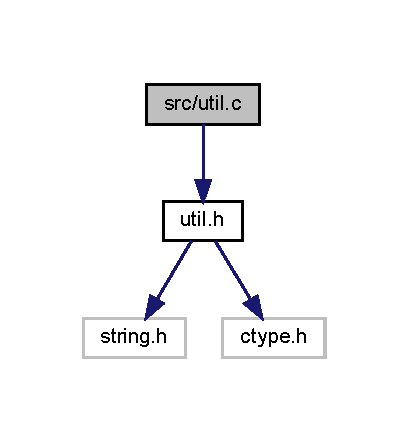
\includegraphics[width=196pt]{util_8c__incl}
\end{center}
\end{figure}
\subsection*{Functions}
\begin{DoxyCompactItemize}
\item 
char $\ast$ \mbox{\hyperlink{util_8c_ac3baffacb2ab73c47735eb93071f52c7}{string\+To\+Lower}} (char $\ast$string)
\end{DoxyCompactItemize}


\subsection{Function Documentation}
\mbox{\Hypertarget{util_8c_ac3baffacb2ab73c47735eb93071f52c7}\label{util_8c_ac3baffacb2ab73c47735eb93071f52c7}} 
\index{util.\+c@{util.\+c}!string\+To\+Lower@{string\+To\+Lower}}
\index{string\+To\+Lower@{string\+To\+Lower}!util.\+c@{util.\+c}}
\subsubsection{\texorpdfstring{string\+To\+Lower()}{stringToLower()}}
{\footnotesize\ttfamily char$\ast$ string\+To\+Lower (\begin{DoxyParamCaption}\item[{char $\ast$}]{string }\end{DoxyParamCaption})}

Returns a string in lower case 
\begin{DoxyParams}{Parameters}
{\em string} & string to be returned in lower case \\
\hline
\end{DoxyParams}

\begin{DoxyCode}
8 \{
9     \textcolor{keywordflow}{for}(\textcolor{keywordtype}{int} i = 0; i < strlen(\textcolor{keywordtype}{string}); i++)
10     \{
11         \textcolor{keywordtype}{string}[i] = tolower(\textcolor{keywordtype}{string}[i]);
12     \}
13 
14     \textcolor{keywordflow}{return} string;
15 \}
\end{DoxyCode}

%--- End generated contents ---

% Index
\backmatter
\newpage
\phantomsection
\clearemptydoublepage
\addcontentsline{toc}{chapter}{Index}
\printindex

\end{document}
